\documentclass{article}
\usepackage[utf8]{inputenc}
\usepackage{biblatex} 
\usepackage{amsmath}
\usepackage{amsfonts}
\usepackage{amssymb}
\usepackage{amsthm}
\usepackage{graphicx}
\usepackage{array}
\usepackage{multirow}
\usepackage{booktabs}
\usepackage{subfig}
\usepackage{physics}
\usepackage{gensymb}
\usepackage{dsfont}
\usepackage{caption}
\usepackage{dirtytalk}

\usepackage{subcaption}


\usepackage{tikz}
\usetikzlibrary{shapes.geometric, arrows}


\usepackage[margin=1.65in]{geometry}
\usepackage[skip=6pt plus1pt, indent=20pt]{parskip}

\addbibresource{report.bib}
\bibliography{report.bib}
\usepackage[nottoc]{tocbibind}


\newtheorem{theorem}{Theorem}[section]
\newtheorem{defn}[theorem]{Definition} 
\newtheorem{cor}[theorem]{Corollary}
\newtheorem{alg}[theorem]{Algorithm}
\newtheorem{example}[theorem]{Example}
\newtheorem{lemma}[theorem]{Lemma}
\newtheorem{prop}[theorem]{Proposition}

\title{Understanding the Behaviour of Reinforcement Learning Agents in Cyber Defence}
\author{Hannah Harrison }
\date{August 2023}




\begin{document}

\maketitle

\vspace{1cm}

\begin{center}
    
A dissertation submitted to the University of Bristol in accordance with the requirements for award of the degree of MSc Mathematics of Cybersecurity in the Faculty of Science.

\end{center}

\newpage

\vspace{8cm}
\begin{center}
  \textbf{ \Large Declaration of Authorship}
  \vspace{0.5cm}

I declare that the work in this dissertation was carried out in accordance with the Regulations of the
University of Bristol. The work is original, except where indicated by special reference in the text, and no part of the dissertation has been submitted for any other academic award. For all ideas taken from other sources (books, articles, internet), the source of the ideas is
mentioned in the main text and fully referenced at the end of the report. All material which is quoted essentially word-for-word from other sources is given in quotation marks and referenced. Pictures and diagrams copied from the internet or other sources are labelled with a reference to the web page or book, article etc. Any views expressed in the dissertation are those of the author.


\end{center}




\newpage

\vspace{8cm}
\begin{center}
  \textbf{ \Large Abstract}

    \vspace{0.5cm}

The use of DeepRL techniques in training autonomous agents to defend cyber networks is gaining popularity. However, such methods are essentially `black boxes', making agents difficult to trust, understand and verify. An emerging field of research attempts to provide explanations for the decisions of RL agents, and in this paper I review the achievements and limitations of these studies. Research from the cognitive sciences indicates that human understanding is fundamentally linked to causal relationships, yet few methods have been proposed which use causal models to generate explanations. Thus, in this paper, I explore a mechanism which wields a \textit{structural causal model} \cite{pearl2009causality} to derive local, post-hoc explanaions of RL agent actions and specifically adapt this for cyber defence applications. This model is tested using the cyber simulator YAWNING TITAN, and evaluated through an example network defence scenario to demonstrate the insights which can be derived.


\end{center}




\newpage 

\tableofcontents
\pagebreak

\section{Introduction and Motivations}

Given the exponential growth and increased usage of data in the modern world, the need for its protection from theft and damage has become essential. Malicious attacks on cyber networks are becoming increasingly sophisticated and complex. This, combined with the rise in cloud services and the influx of private data from Internet of Things (IoT) devices, means that the defence scenario is becoming more and more impenetrable. Coordinated attacks can compromise multiple hosts in quick succession once inside a network, necessitating a robust threat detection and response system. 

In \cite{dhir2021prospective}, the authors discuss examples of new malicious tools that current defenders can’t rapidly adapt to, and argue that we need new advanced cyber-defence methods to counter them. They propose the rapid introduction of reinforcement learning (RL) for the purpose of active cyber defence. Indeed, the use of RL techniques in training agents to defend against malicious attacks on networks is gaining popularity, and a large proportion of recent progress in this area is attributable to  DeepRL, which utilises deep learning techniques in the training of agents. An up-to-date survey of such techniques is given in \cite{sewak2022deep}, in which the authors emphasise the significant performance improvements DeepRL techniques have yielded in many complex, real-world security applications. Since policies are learned by continually observing and interacting with the environment, the training of  DeepRL agents requires large amounts of online data collection, which can be computationally expensive. One approach to mitigate this is to train in a simulated environment from which the learned policy can then be shifted to the desired environment with little additional training. As such, this work utilises data drawn from a novel cybersimulator, YAWNING TITAN \cite{YT}.

Despite the performance enhancements yielded by DeepRL techniques, it is often difficult to explain the decisions made by such agents due to the `black box' nature of many deep learning methods \cite{PearlMackenzie18}. This lack of explainability can make algorithms difficult to trust, understand and verify, yielding both ethical and practical concerns. Such problems are highlighted when an agent behaves in an unpredictable manner, which can occur when the target environment is outside of the `training bounds' of the agent, i.e. when the target environment is significantly different to the environment in which the agent was trained. This problem causes significant concern in highly dynamic domains such as the defence of cyber networks, in which the environment and attack vectors are prone to change quickly and frequently. Further, the use of simulations to develop DeepRL agents as mentioned above can also cause the training and target environments to differ. Hence an improvement in the explainability of DeepRL agents could help in the understanding and predictability of the algorithm's behaviour. Moreover, DeepRL models are complex to debug \cite{heuillet2021explainability}, and an explainable model could aid in fixing problems more quickly and accelerate new development in RL methods. 

The emerging area of research which focuses on explaining the decisions of RL agents has been coined Explainable Reinforcement Learning (XRL) and is a relatively new subfield of Explainable AI (XAI) research. Much progress in XRL has been achieved by making use of existing XAI methods \cite{wang2022causal}, and in particular \cite{heuillet2021explainability} provides a review of recent developments in XAI and makes suggestions on how these techniques may be adapted to DeepRL policies. However, most of these studies take an associational perspective; `importance' is measured in terms of the correlation between state features and the subsequent action. As follows from the commonly accepted notion that \say{correlation does not imply causation} (\cite{PearlMackenzie18}), features which are highly correlated with a given action may not actually be real `causes', resulting in incorrect explanations. This can degrade trust in the system.


Many researchers in the field of XAI argue that `better' explanations (in terms of human understandability and reliability) can be extracted from models by considering causality \cite{madumal2020explainable}. While a majority of machine learning models focus on correlations found between features in the training data, these correlations can be coincidental and what we are actually interested in is the causal effect of one variable on another \cite{PearlMackenzie18}. The branch of science devoted to understanding such causal relationships is known as causality, and it is widely accepted that human cognition and understanding relies on such relationships. The main aim of this research is to explore the application of causal models to explain local decisions made by deep RL agents, and in particular how such methods can be applied in the context of cyber threat response. As such, the contributions of this paper are twofold.  Firstly, recent work in XRL is reviewed with a focus on post-hoc explanations and causality. Secondly, significant alterations are made to adapt the importance calculation method in \cite{wang2022causal} to suit a cyber defence simulation environment featuring a finite action space and a mixture of binary and discrete observations.

%This is done by calculating the importance of individual features of the state space on the actions taken by the RL agent via a structural causal model. The idea of causal state and temporal importance for generating explanations has been explored in \cite{wang2022causal}, however the novel simulation environment considered in this work presents unique challenges. The contributions of this paper are twofold. Firstly recent work in XRL is reviewed with a focus on post-hoc explanations and causality. Secondly, significant alterations are made to adapt the importance calculation method in \cite{wang2022causal} to suit a cyber defence scenario featuring a finite action space and a mixture of binary and discrete observations.

The report will be structured as follows. Section 2 will cover the relevant background material, including the general setup of a reinforcement learning problem, and an introduction to causal diagrams, structural causal models and counterfactual reasoning. Section 3 will be devoted to a review of the relevant work in the field of XRL, including both associational and causal methods. In Section 4, I will introduce the cybersimulator to be used in this work; YAWNING TITAN. This is highly configurable, and so some time will be spent specifying the parameters of the environment, and formulating the problem as an MDP. Section 5 will outline the methodology for calculating importance weightings and Section 6 the results, with an expository example. Conclusions and further work will be discussed in Sections 7 and 8 respectively. 
 

\pagebreak


\section{Essential Background}

\subsection{Reinforcement Learning}

\subsubsection{Fundamentals}

Reinforcement Learning (RL) is a subfield of machine learning that deals with an agent's ability to learn and make decisions by interacting with an environment. Inspired by behavioral psychology and the concept of trial and error learning \cite{gershman2017reinforcement}, RL aims to train an autonomous agent to maximize its cumulative reward by making informed decisions based on past experiences. 

\begin{figure}[htp]
    \centering
    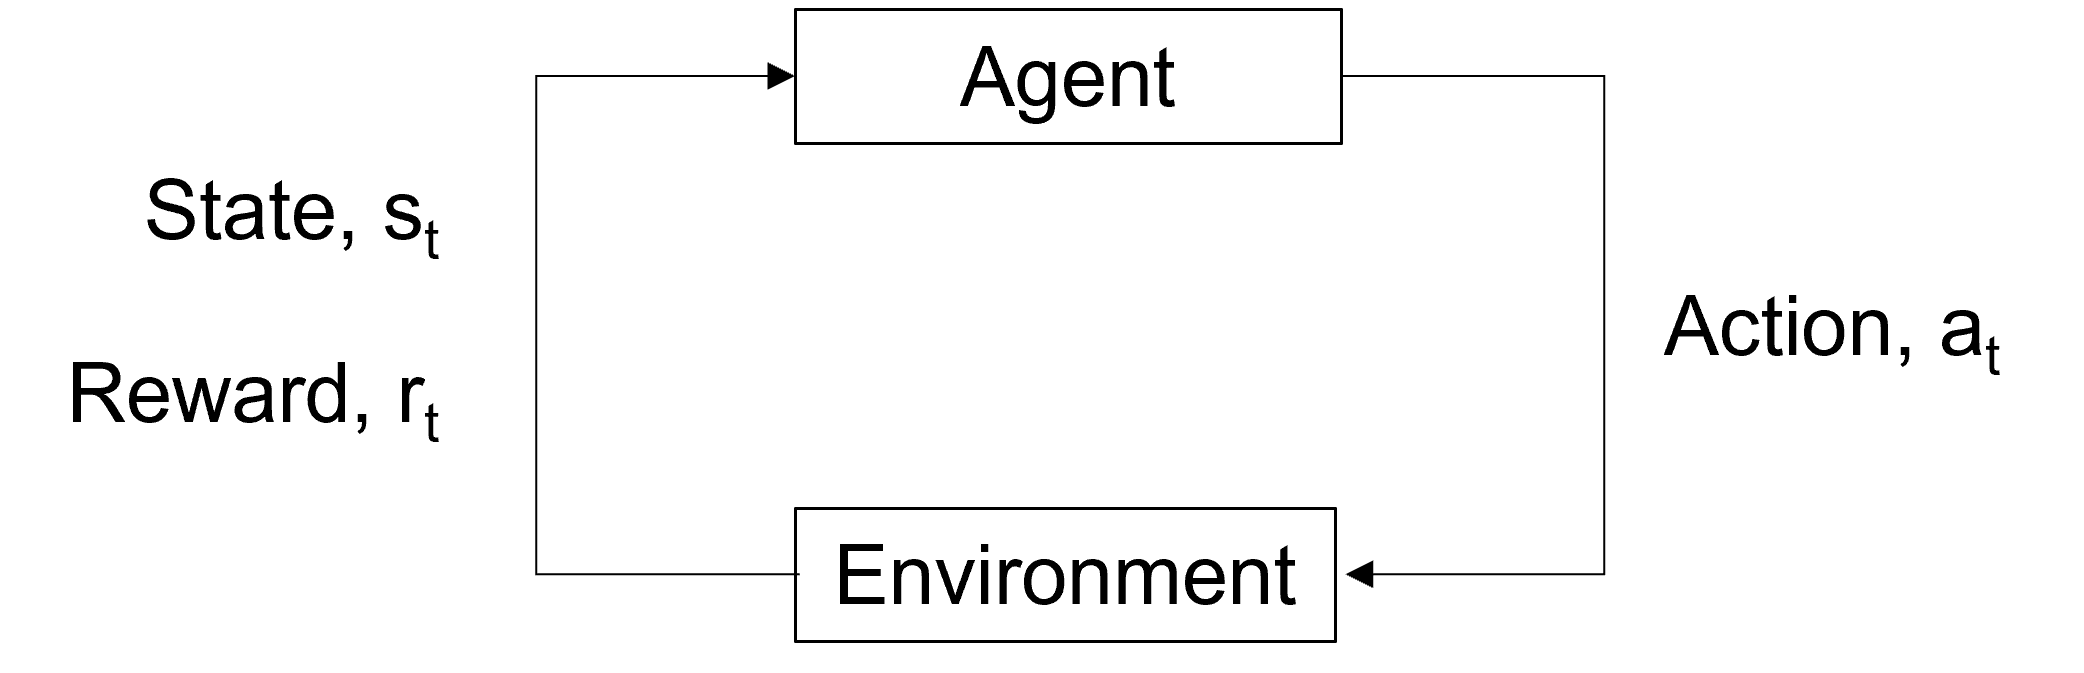
\includegraphics[width=0.8\textwidth]{Images/Reinforcement loop.png}
    \caption{The reinforcement loop. An agent interacts with the environment by observing its current state and applying an action based on this observation. The agent then receives a reward, observes the resulting new state, and the process continues. \footnotemark}
    \label{fig:RLloop}
\end{figure}

\footnotetext{Figure inspired by Figure 3.1 in \cite{sutton2018reinforcement}. }

\noindent The fundamental process loop for the RL problem is given in Figure \ref{fig:RLloop}. In particular, at a given time step, $t = 0,1,2,...$, the agent observes the current state of the environment $s_t$, and based on this, executes an action $a_t$. It then observes a reward $r_t$, along with a new state $s_{t+1}$. This process continues ad infinitum, or until an end state, or maximum number of time steps is reached. The  environment is usually modelled as a Markov Decision Problem (MDP), and the elements of such a problem, along with their notations for use in this paper, can be summarised as follows. 

\begin{itemize}
    \item \textbf{Agent} - The learner or decision maker. It is the entity responsible for taking actions in the environment based on its current state and the available information.
    \item \textbf{Environment} - The external context with which the agent interacts. 
    \item \textbf{State, $\mathbf{s_t}$} - A representation of the variables in the environment observed by the agent at time $t$. This takes values in a state space $\mathcal{S}$, comprising of all possible states. The state space can be finite or infinite depending on the variables involved.
    \item \textbf{Action, $\mathbf{a_t}$} - the method by which the agent interacts with the environment. We refer to the set of available actions as the action space, $\mathcal{A}$, which may depend on the current state. Hence we denote the set of available actions at a state $s$ by $\mathcal{A}(s)$.
    \item \textbf{Policy, $\mathbf{\pi(a_t|s_t)}$} - A function mapping states to actions, which acts as the strategy used by the agent to select a decision based on the current state.   
    \item \textbf{Reward, $\mathbf{r_t}$} - The output of a reward function, $R_t(a_t,s_t)$, which acts as feedback to the agent.
    
\end{itemize}

\noindent The aim of an RL agent is to learn the optimal policy, $\pi^*(a|s)$, which maximises the expected cumulative reward, $\mathbb{E} \left[ \sum^{\infty}_{t=0}R_t(a_t,s_t) \right]$. To illustrate these concepts, we consider a classic `grid world' style environment in Example \ref{ex:gridworld}, inspired by Section 1 of \cite{sutton2018reinforcement}.

\begin{example}

The grid world environment is a 4x4 array of 2D spaces, as shown in Figure \ref{fig:Gridworld}. Here, the agent is an insect, whose goal is to reach the berries by traversing the squares, without encountering the fire or insect spray. The state of the environment in a given time step is the square occupied by the insect, and the available actions are up, down, left and right. Reaching the berries incurs a positive reward, whilst encountering the bug spray or fire results in a negative reward. The insect begins by taking random actions and observing the rewards associated with them. Thus, since the goal is to maximise the reward, over time the insect learns a policy, instructing which action to take based on its current position, in order to reach the berries whilst avoiding the obstacles. 

\label{ex:gridworld}
\begin{figure}[htp]
    \centering
    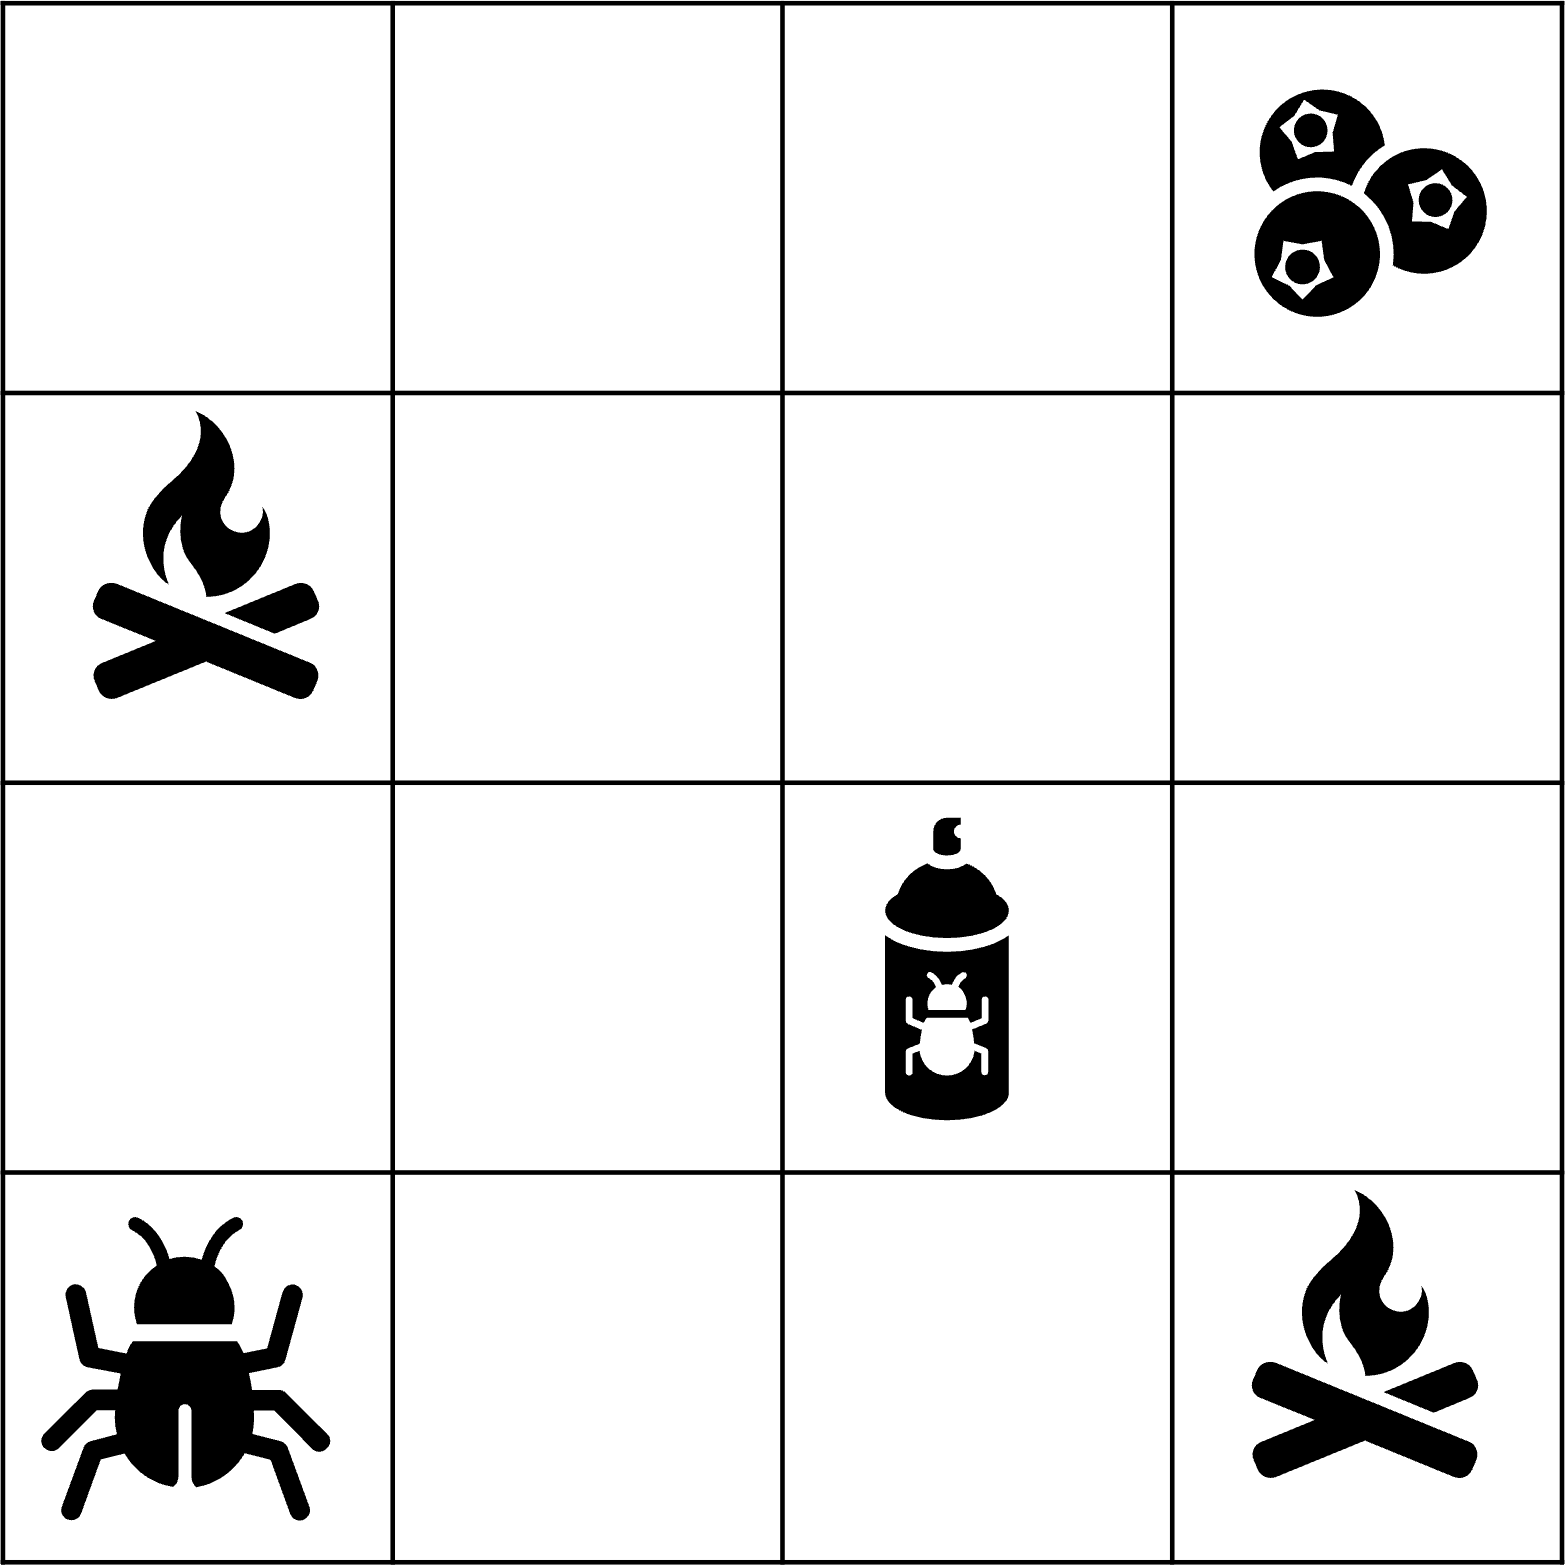
\includegraphics[width=0.4\textwidth]{Images/Gridworld.png}
    \caption{The grid world environment from Example \ref{ex:gridworld}, in which a reinforcement learner takes the role of an insect attempting to reach the berries whilst avoiding obstacles. }
    \label{fig:Gridworld}
\end{figure}

\end{example}

\noindent There are many different algorithms in use for reinforcement learning, typically categorized into two main classes; value-based and policy-based. Value-based methods, such as Q-learning, learn the value of states and use this to infer an optimal policy. In particular, they define a value function, 
\begin{align}
\label{eq: value function}
    V_{\pi}(s) = \mathbb{E}[G_t | S_t],
\end{align}

\noindent which yields the expected value of the total cumulative reward from time step $t$ onwards (denoted $G_t$) starting at state $s$ and following the policy, $\pi$, thereafter. Due to the onerous task of summing all rewards an agent can receive starting at each state, the state values are usually calculated recursively via the Bellman equation. This is defined in section 3.7 of \cite{sutton2018reinforcement}, where the authors give a comprehensive explanation of value-based RL methods.

Policy-based methods, on the other hand, are focused on learning the optimal policy directly, which is often achieved via gradient descent. Specifically, policy-gradient methods learn a stochastic policy by iteratively updating action probabilities with respect to an objective function;

\begin{align}
\label{eq: objective function}
    J(\theta) = \sum_{\tau} \mathcal{P}(\tau;\theta) R(\tau), \hspace{0.5cm} \mathcal{P}(\tau;\theta) = \prod_{t = 0}^{\infty} \mathcal{P}(s_{t+1}|s_t, a_t)\pi_{\theta}(a_t | s_t).
\end{align}
Here, $\tau$ denotes a trajectory through the state space and $R(\tau)$ the cumulative expected reward from that trajectory. $\mathcal{P}(\tau;\theta)$ gives the probability of the trajectory based on the state transition probabilities $\mathcal{P}(s_{t+1}|s_t, a_t)$ and policy $\pi_{\theta}(a_t | s_t)$, which gives the probability of taking action $a_t$ at state $s_t$. Updates are performed via gradient ascent, increasing the probabilities of actions that lead to higher cumulative rewards. The details are beyond the scope of this report, however the interested reader should see Chapter 13 of \cite{sutton2018reinforcement}.

One of the most popular policy gradient methods, currently hailed as state of the art, is proximal policy optimisation (PPO) \cite{schulman2017proximal}, which aims to improve training stability by bounding the change in action probabilities in any single iteration. This has resulted in high empirical performance on RL benchmarks whilst being general purpose enough for a wide variety of applications \cite{ppofacts}, making PPO a very popular choice in a variety of contexts. 


\subsubsection{DeepRL}

Many popular reinforcement learning algorithms now use neural networks within the policy learning process, and such techniques are known as deep reinforcement learning. PPO is an example of such a technique, and utilises two deep neural networks; one handling action selection from the input observation (the actor), and one which determines the 'value' of the action by predicting the future rewards. As such, PPO is termed an `actor-critic' method \cite{schulman2017proximal}.

This trend towards the use of deep learning algorithms is due to their ability to take very large, unstructured input data. This reduces the need for manual engineering of the state space, and allows reinforcement learning to be used on a wider range of more complex problems. However, this use of neural networks comes with a loss transparency; the focal issue in this report.


Due to being a very popular, yet complex DeepRL technique, along with its integration in the RL library Stable Baselines3 \cite{stable-baselines3}, PPO will be the main training algorithm used in this research. 



\subsection{Causality}

Causality, the relationship between cause and effect, has been a central concept in human understanding since ancient times. Its origins can be traced back to ancient Greek philosophy and the ponderings on the reasons behind observed changes in the physical world \cite{pearl2018book}, but it was not until the 20th century that causal inference methods emerged in statistics and experimental design. However, it is difficult to arrive at a universal definition of a cause, let alone a universal framework for discovering causal structure because the concept of causality is complex, and subject to interpretation and context-dependent considerations \cite{xie2019causality}.

One approach used in time series analysis, known as Granger causality, assesses causal effects in terms of whether one time series can predict or provide valuable information about another time series. This formulation of causality is used in many applications, such as determining the impact of interest rates on economic growth in economics and analysing functional connectivity between different regions of the brain in neuroscience.
However, while Granger causality is useful for exploring temporal relationships in time series data, it falls short in capturing the directionality and qualitative strength of causal connections. Instead, we will consider Judea Pearl and Joseph Halpern's  Structural Causal Model (SCM) \cite{halpern2005causes1} framework, which provides a formal approach to understanding causality through directed acyclic graphs.


\subsubsection{Causal diagrams}
This section formalises the causality concepts used in this work, with much of the following background originating from \cite{halpern2005causes1} and \cite{halpern2005causes2}. I provide a minimal background including only the definitions relevant to this work, and direct the interested reader to \cite{pearl2009causality} for a more thorough discussion. 

\begin{defn}
 (Causal network) \cite{pearl2018book}

 \noindent A causal network is a probabilistic graphical model for a data generating process. Let $\mathcal{V} = {V_i, i = 1,...,n}$ be a set of variables. Each variable is represented by a node in the graph, and a directed edge from a variable $V_i$ to another variable $V_j$ implies that $V_i$ is a cause of $V_j$. In particular, a change in $V_i$ results in a change in $V_j$ when all other variables are held constant. 
\end{defn}

\noindent Within a causal network, we distinguish between two types of variable; exogenous and endogenous. An endogenous variable is one whose value is determined by other variables in the model, whereas as exogenous variable is not explained by other variables. In particular, exogenous variables have no explicit cause within the model and as such have no directed edges leading to them in the causal graph.

To clarify these concepts, let's consider an example.

\begin{example}
\label{ex:causal_diagram}
 
Consider the variables: Altitude, $A$, Temperature, $T$, Season, $S$ and proportion of hikers catching Hypothermia $H$. From these, we can produce a causal diagram encoding the cause and effect relationships as shown in Figure 
\ref{fig:hypothermia_diagram}. We assume that all causal links are present in the construction of the diagram. In particular, the absence of a directed arrow between, for example, nodes $A$ and $H$, indicates the implicit assumption that the entire causal effect of $A$ on $H$ is through $T$.
     
\begin{figure}[htp]
    \centering
    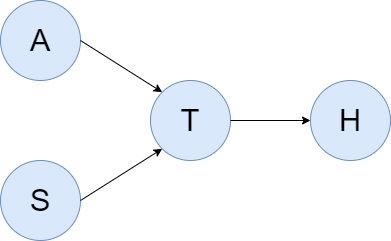
\includegraphics[width=0.4\textwidth]{Images/Causal example-Page-1.drawio.png}
    \caption{A causal diagram for the hypothermia situation. Arrows indicate directed causal relationships. From left to right the nodes represent the exogenous variables; altitude and season, followed by the endogenous variables; temperature and proportion of hypothermia cases. }
    \label{fig:hypothermia_diagram}
\end{figure}

\noindent In Figure \ref{fig:hypothermia_diagram} there is an arrow directed from $A$ to $T$, as a change in altitude affects the temperature distribution. However, there is no arrow between altitude and season, as clearly a change in altitude does not change which season it is. In this model, $A$ and $S$ are exogenous, as they have no cause within the model, whilst $T$ and $H$ are endogenous. 

\end{example}


\noindent The topology of a causal graph is usually referred to as its skeleton, and this can either be derived from background knowledge, or learned using a causal discovery mechanism. Examples of such methods include the PC algorithm \cite{spirtes2000causation} and non-Gaussian methods such as LiNGAM \cite{shimizu2006linear}. For the purpose of this work, we will assume a causal model is given. 

Using this framework, we can give a more precise definition of a cause. 

\begin{defn} 
(Direct cause) \cite{pearl2018book}

    \noindent We say that a variable, $V_i$, is a parent or `direct cause' of another variable, $V_j$, if $V_i$ is  connected to $V_j$ by a series of directed edges in the causal graph.
\end{defn}


\noindent For example in the setting of Example \ref{ex:causal_diagram}, we can say that the season is a direct cause of hikers catching hypothermia. This makes intuitive sense as we would expect higher rates of hypothermia in the winter. 

Causal diagrams alone are a useful tool for visualising causal relationships, but they can also aid in quantifying the causal effect of one variable on another when paired with what is know as a structural causal model.

\subsubsection{Structural Causal Models}

\label{sec: SCM}


\begin{defn} (SCM) \cite{YT}

\noindent Let $\mathcal{V} = \{V_i \hspace{1mm}| i = 1,...,n\}$ be a finite set of endogenous variables and $\mathcal{U} = \{U_i \hspace{1mm}| i = 1,...,m\}$ be a set of exogenous variables. We define a structural causal model (SCM) as the quadruple ${V,U,\mathcal{R},\mathcal{F}}$, where $\mathcal{R}$ is a function specifying the range of each variable. $\mathcal{F} = \{f_i, i = 1,...,n\} $ denotes a set of functions specifying each endogenous variable in terms of the other variables in $\mathcal{U} \cup \mathcal{V}$. 
\end{defn}

\noindent Each SCM is associated with a causal diagram, and the functions in $\mathcal{F}$ encode the causal relationships between the variables. In particular, we can write: 
\begin{align}
    V_i = f_i(\mathcal{P}_i, U_i), \hspace{0.5cm} i = 1,...,n 
\end{align}
\noindent where $U_i \subseteq \mathcal{U}$ and $\mathcal{P}_i$ denotes the parents of the variable $V_i$ in the causal graph. 

An SCM can be used for calculating causal interventions (changing the value of a variable to assess its effect on another) and to properly denote this, we need to introduce $do$-calculus \cite{huang2012pearl}. The $do(.)$ operator is used to signal the intervention, with $do(V_i = x)$ representing setting the value of variable $V_i$ to $x$ regardless of any observational data, and any edges into $V_i$ in the causal network. The structural equations in the SCM can then be used to calculate the change in the values of the other variables of interest resulting from the intervention. For more detail on this see \cite{pearl2009causality}. Such interventions form the basis of scientific experimentation, for example assessing the effect of doubling the dose of a drug (initially $D=1$), on the chance of surviving a disease ($S)$, while all other relevant variables are held constant, can be expressed mathematically as:
\begin{align}
    \mathbb{P}(S| do(D = 2)).
\end{align}

\noindent It is important to clarify that the do-operation is distinct from conditioning in statistics. Correlation between variables means that conditioning on a variable gives information about its parents, whereas the do-operation is independent of the other variables.

True structural equations are in general difficult to discern, and so in most cases require approximation. Many approximation methods have been explored for this purpose in the literature, including multiple regression \cite{madumal2020explainable}, decision trees \cite{madumal2020distal} and neural networks \cite{wang2022causal}, as will be discussed in Section 3.2. For the purpose of this work, we will use logistic regression, due to the finite nature of the variables included in the causal model presented in Section 4.2.


\subsubsection{Counterfactual reasoning}
Counterfactual reasoning is the top `rung' of Pearl's hierarchy of causal reasoning, the `ladder of causation' \cite{pearl2018book}, and is where SCMs become most useful. A counterfactual is a causal situation of the form `if X had not happened, would Y have happened?'. For example, in the setting of Example \ref{ex:causal_diagram}, we could ask, `what would the effect of an increase of 100m in altitude have had on the prevalence of hypothermia?'. Note that this is different from an intervention, as we are not actually altering the altitude, just considering what would have happened in an alternate world in which we did.  There is much research which suggests that counterfactuals form a fundamental part of human understanding of the world \cite{madumal2020distal}, and in \cite{madumal2020explainable}, human experiments demonstrate that the availability of counterfactual explanations for agent actions improves on both task prediction and explanation satisfaction compared to observing the agent alone. 

Formally, suppose that the observed state is $X_t = x$ and corresponding outcome is $Y_t = y$, but we are interested in the counterfactual question: what would have been the value of $Y_t$ if $X_t$ had had some other value, $x'$? This counterfactual outcome can be denoted as:
\begin{align*}
    Y_{t, X_t = x'} | X_t = x, Y_t = y.
\end{align*}

We can now appreciate the utility of an SCM, as we can use it to perform counterfactual reasoning via interventions. We do this by first recovering the value of the exogeneous variables $\mathbf{U = u} $ via the structural functions, then calculating the counterfactual outcome as $Y_t|do(X_t = x')$. This is demonstrated in Example \ref{ex:counterfactual calculation}. 
\begin{example}
\label{ex:counterfactual calculation}

Once again we return to the setting of Example \ref{ex:causal_diagram}. Suppose that we know that in Winter, the proportion of hypothermia cases is 0.1 \%. Suppose also that we have learnt the structural functions $H = -0.2T + 0.5$  and $ T = -0.01A -S +20$. Here $S$ is given values $0,1,2,3$ corresponding to Summer, Spring, Autumn and Winter respectively. We are interested in what would happen if the season was Spring. 

First, we use the known values to recover the values of the exogenous variable $A$. We have $T = - 0.01A - 3 + 20 $, which we can substitute into the the equation for $H$, giving $0.1 = -0.2(-0.01A +17) + 0.5$. Hence we have $A = 1660 $m. 


Now, we can calculate the counterfactual outcome as $H | do(S = 1) $ using the structural equations. $T = -0.01 \times 1660 -1  + 20 = 2.4 \degree C$. $H | do(S = 1) = 2.4 \times -0.2 + 0.5 = 0.02 \%$. 

\end{example}

\noindent 
Note that whilst in Example \ref{ex:counterfactual calculation} we consider linear structural equations for ease of explanation, linearity is not assumed in general in an SCM. Indeed, the form of the structural equations should be carefully considered to avoid `out of range' values, such as negative probabilities. This kind of counterfactual manipulation is sufficient for the purpose of this work, however the interested reader should see \cite{pearl2009causality} for a more in depth introduction.

\pagebreak

\section{Literature Review}
%XAI, XRL, split papers to be included into categories
% Review other papers, present some of their maths with figures etc...
% ------------------------------------------------------
In this section, I give a high level review of the current literature in XRL, with the aim of putting this work in context and giving intuition on what is meant by explainability in the context of machine learning.  

\subsection{What is explainability?}
\label{sec:explainability}

Despite many papers in the field presenting their own views of what is meant by an explainable RL method, these are often highly application specific, and a clear consensus has not been reached, nor have any standard criteria been developed. This poses a great challenge, as it hinders both the understanding of XRL work, and the development of evaluation metrics for comparing techniques \cite{qing2022survey}. 

Many XRL papers are focused around a key definition of either interpretability or explainability. In \cite{miller2019explanation}, interpretability is specified as the extent to which a person can understand a model. On the other hand, the authors of \cite{kim2016examples} recognise interpretability in terms of whether one can consistently predict a result. Considering explainability, some papers such as \cite{wang2022causal} present the concept as a post-hoc property concerning whether the mechanism by which decisions were made can be understood, while others (e.g. \cite{madumal2020explainable})  define it as the ability to provide intuition about individual model predictions. A recent work, \cite{vouros2022explainable}, has provided a distinction between explainability and interpretability based on the common usage of the terms, which has been adopted in subsequent works, including \cite{glanois2021survey}. In particular, the authors suggest that while interpretability concerns the passive ability to utilise the properties of a model to provide explanations, explainability is an active notion corresponding to external methods which provide insights on inner workings of the RL model. I.e. there are two possible architectures of XRL technique; we can either design an RL method in which the agent's decisions are transparent enough to be understood by a human as is, or we can construct a mechanism capable of pairing human-readable logic with an agent's decisions. 

Note that both concepts, interpretability and explainability, may be conditional on the audience. Indeed, what constitutes a good explanation may vary considerably for an  a domain expert, end-user, or a legislator. In this report we will discuss examples with a variety of intended audiences, but focus the main research on domain experts, as they are the most likely observer of autonomous cyber defence agents. 


\subsection{Taxonomy of research}

\begin{figure}[htp]
    \centering
    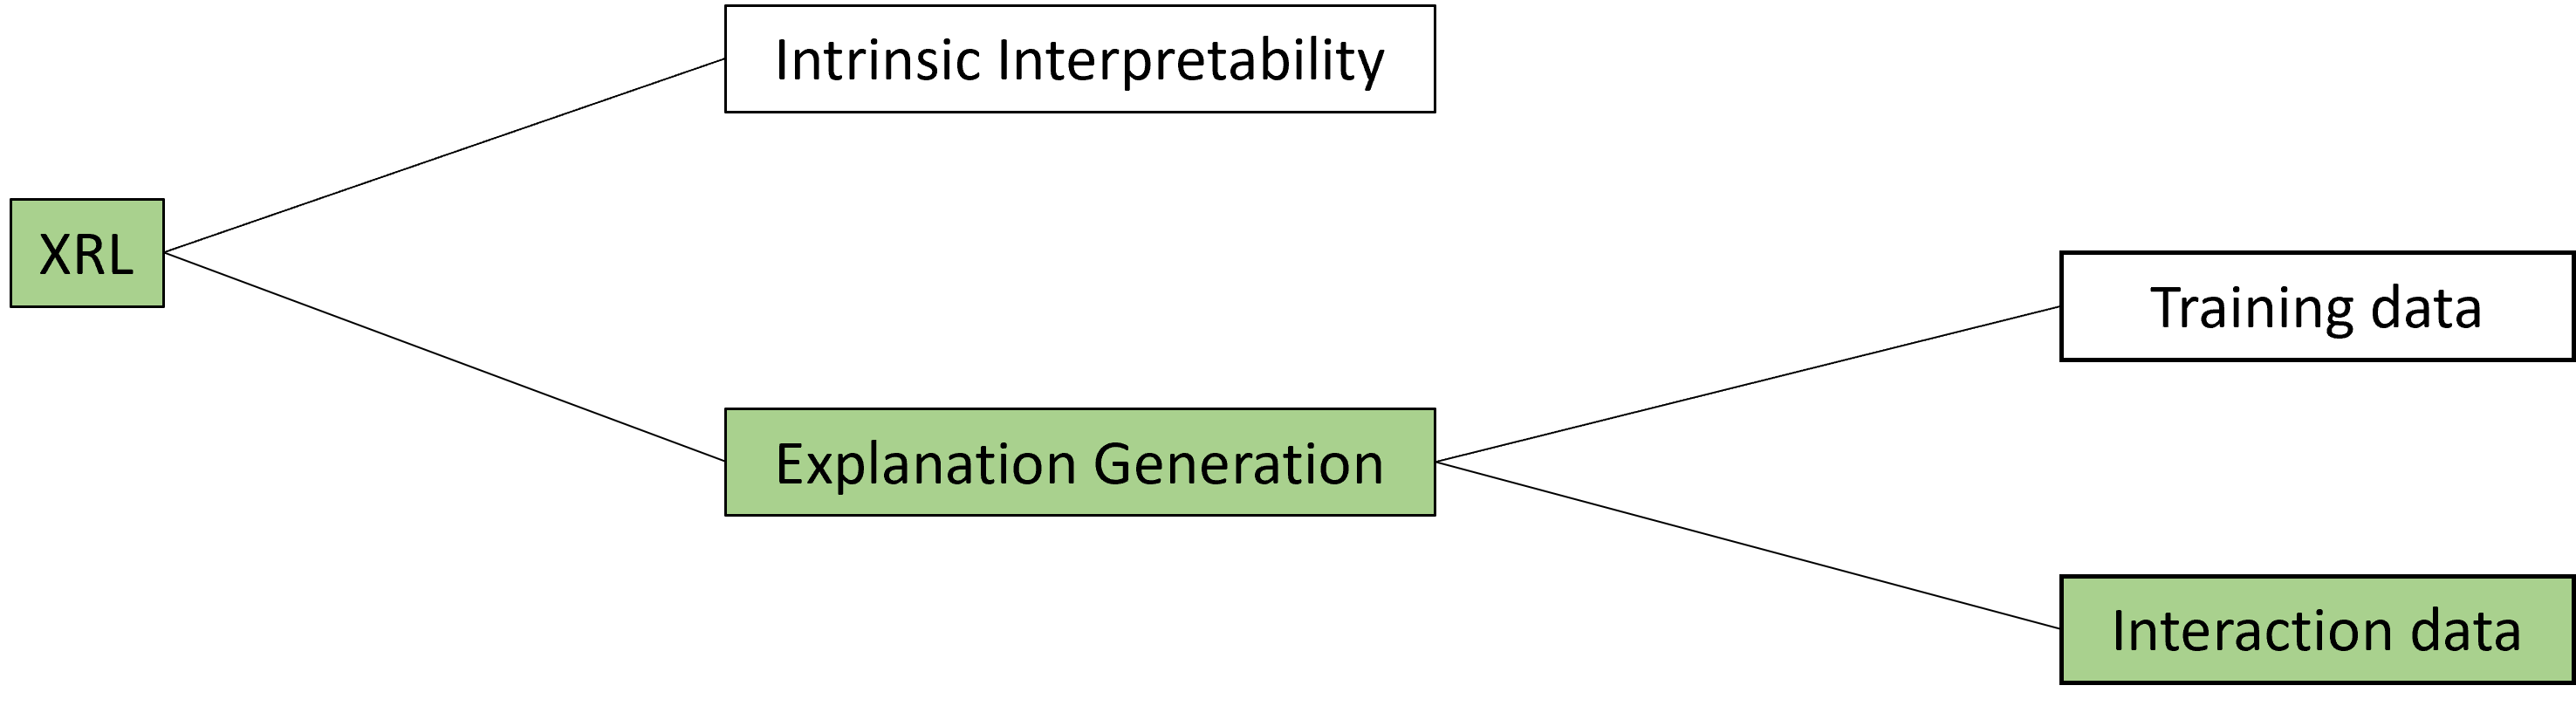
\includegraphics[width=0.8\textwidth]{Images/XRL taxonomy.png}
    \caption{A proposed taxonomy of XRL research. The green indicates the class of the method featuring in this report.}
    \label{fig:xrl_taxonomy}
\end{figure}

XRL research can be broadly split into two main classes according to the definitions of interpretability and explainability discussed in Section \ref{sec:explainability}; intrinsically explainable algorithms and post-hoc explanation generation. The former class includes all techniques which are inherently transparent in the sense that a human can understand the decision mechanism by inspection of the model. Examples of such techniques include decision trees \cite{pmlr} and rule-based systems \cite{sewak2022deep}. However, whilst these methods are often able to achieve a high performance in specific problems, it is generally the case that the more powerful and flexible a reinforcement learning algorithm is, the more opaque it becomes \cite{sewak2022deep}. Particularly in the case of DeepRL, many of the most `general purpose', high performance algorithms (such as DQN, PPO and A2C) are essentially black boxes. This trade-off between performance and interpretability is well recognised in the literature, although is referred to by different names, for example accuracy-interpretability trade-off \cite{rudin2019stop}, readability-performance trade-off \cite{dovsilovic2018explainable} and interpretability-scalability trade-off \cite{glanois2021survey}. 


Although there are arguments for focussing research on intrinsic interpretability (especially in the case of high stakes decisions, for example see \cite{rudin2019stop}), the dominance of complex, model-agnostic algorithms in RL has lead to a shift in attention towards post-hoc methods of explanation. These methods can be further classified into two main categories based on the stage at which the explanation generating model is fitted, as indicated by the proposed taxonomy in Figure \ref{fig:xrl_taxonomy}. Explanation models can be trained either using replay data consisting of state-action pairs collected during the agent's training, or with data drawn from post-training interactions with the agent. 

The former class of explanation-generating techniques train a surrogate explanation model alongside the RL agent using replay data consisting of state-action pairs collected during the agent's training. This enables the identification of the prominent features which influenced the training of the policy. An example of such a technique is the reward decompostion method presented in \cite{juozapaitis2019explainable}. Here, the reward collected in each time step is partitioned into sub-components based on distinct goals, and the surrogate model aims to identifty which sub-component has the greatest influence in the agent's learning of which action to take at a specific state. In this way, explanations can be provided based on the specific objective of the agent at that time. For example, if in the gridworld setting of Example \ref{ex:gridworld}, we impose a penalty for each time step the insect hasn't reached the berries, we can explain a specific movement as motivated either by taking the shortest path to the berries, or avoiding an obstacle. This kind of method works best in scenarios where the rewards naturally fall into distinct classes, such as in the Starcraft II domain exemplified in the source paper. 

The latter class of explanation-generation techniques differs from the previous in that they utilise data drawn from post-training interactions with the agent, rather than being trained alongside. In this way, explanations can be derived without the need to re-train an RL agent to collect the required replay data, or implement surrogate model architecture before training commences. Many techniques in this class stem from saliency mapping techniques originally introduced for supervised learning \cite{simonyan2013deep}, and such approaches in XRL have been shown to be effective for explaining the decisions of RL algorithms trained on image data. These methods work by generating a type of heat map which highlights the pixels which have the greatest influence on the agents' decisions. An interesting example in \cite{greydanus2018visualizing} presents a perturbation-based method for producing saliency maps for RL agents playing Atari2600 games. The fundamental idea is to apply a perturbation to an image that removes information from one pixel without adding any new information, and compare the agent's decisions based on the original and perturbed image. This is then repeated for each pixel in turn and the information gathered presented as a heat map overlaid on the original image so that the observer can easily see the important features. An example saliency map for the Atari game `Space Invaders' (reproduced from \cite{greydanus2018visualizing}) is shown in Figure \ref{fig:saliency map}, and illustrates the most important features for an RL agent's decision of direction to aim in order to hit enemies.

\begin{figure}[htp]
    \centering
    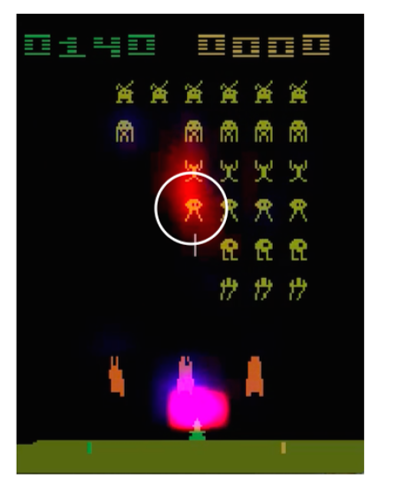
\includegraphics[width=0.3\textwidth]{Images/saliency map.png}
    \caption{A saliency map for the Atari game `Space Invaders', reproduced from \cite{greydanus2018visualizing}. The red indicates the salient pixels in the RL agent's decision of which direction to aim in.}
    \label{fig:saliency map}
\end{figure}


Saliency map methods have also been adapted for non-image data, and an example of such a technique is presented in \cite{olson2021counterfactual}, where features of the observation space are incrementally altered to determine the minimal change necessary to induce a change in action. Although we cannot produce such a clear visualisation as a pixel importance map, this information can then be used to provide feature importance based explanations of specific actions, as elements of the state space which require a less significant change likely had more influence in the agent's choice of action at that time. In this paper, we will take a similar approach in varying features of the state space in order to allow the application of the technique to agents which have already been trained. 



\subsection{Causal explanation methods}

Whilst there are a growing number of papers presenting various XRL techniques, few incorporate causality. Eschewing causality can  facilitate correlation-based errors as discussed in Section 1 and so I will focus the remainder of this section on reviewing the existing examples of causal XRL for local action explanation generation. 


\subsubsection{Action-Influence models}

In what is claimed to be the first appearance of causal models in XRL \cite{madumal2020explainable}, Madumal et al. motivate the necessity of causality within human-focussed explanation generation by citing psychological sources demonstrating that human understanding is inherently driven by cause and effect relationships. The authors aim to address `why' and `why not' questions with regard to specific agent actions, which makes the work unique from other XRL techniques as it uses counterfactuals to provide explanations for events which did not occur \cite{puiutta2020explainable}. 

To achieve this, the structural causal model (SCM) defined in Section \ref{sec: SCM} is extended to encompass agent actions,  a construction which they call an Action Influence Model (AIM). In particular, the actions which correspond to each causal link are identified and instead of just one structural equation for each state variable, $S^{(i)}$, as in an SCM, in an AIM there are multiple — one for each unique action set that influences $S^{(i)}$. A graphical representation of their action influence model for a game scenario (Starcraft II) is given in Figure \ref{fig:action-influence}, where we can see the actions which cause each change are given above the corresponding causal link. 

\begin{figure}[htp]
    \centering
    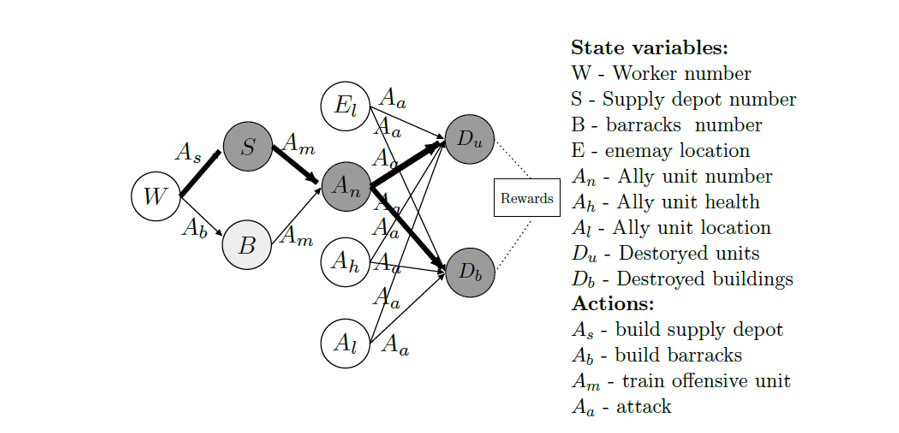
\includegraphics[width=0.8\textwidth]{Images/Action influence.png}
    \caption{An action influence model for the Starcraft scenario, replicated from \cite{madumal2020explainable}. This is an extension of a causal diagram, where the actions corresponding to a cause are given along the causal arrows. The action influence graph is traversed to provide explanations. For example, an explanation for the question `why not take action $A_b$' is given as `Because it is more desirable to do the action $A_m$ to have more ally units ($A_n$) as the goal is to have more Destroyed Units ($D_u$) and Destroyed buildings ($D_b$).' \cite{madumal2020explainable}.
    }
    \label{fig:action-influence}
\end{figure}


\noindent The explanation generation process using an AIM entails three stages.

\begin{enumerate}
    \item \textit{Define an action influence model}.  The qualitative causal relationships between states and actions are represented in the format of an AIM. The authors assume that these relationships are known.
    \item \textit{Learn the structural equations}. Due to the complexity of uncovering the true structural equations that define variable relationships, these are approximated via multivariate regression models learned during the training of the RL agent.
    \item \textit{Generate explanations}. Explanations for specific agent actions are generated by traversing the action influence graph to obtain the corresponding rewards. In particular, the authors define `minimally complete contrastive explanations' which include only variables deemed essential. The explanation for a question of the type `Why not action $A$?' is constructed by simulating the counterfactual scenario that action A had been taken using the structural equations, and comparing this to the actual scenario (hence the term `contrastive'). These explanations are then inserted into a Natural Language Processing (NLP) template to produce human-readable outputs. An example explanation produced in \cite{madumal2020distal} is given in Figure \ref{fig:action-influence}.
\end{enumerate}

\noindent Evaluations of the AIM method show promising results. In a comparison across six RL benchmark domains (using different DeepRL algorithms), the model exhibits reasonable task prediction accuracy and minimal training time \cite{puiutta2020explainable}. In a human study involving a simplified version of the strategy game Starcraft II, the action influence model is compared against giving no additional explanation other than watching the agent, and an explanation generated using an associative model. The assessment considered task prediction by humans, satisfaction with explanations, and trust in the model. Results indicate the action influence model performs notably better in task prediction and explanation satisfaction, though not in trust.

Building on this work, \cite{madumal2020distal} instead produces explanations based on potential future actions. This is achieved using the concept of opportunity chains extracted from their action influence graph, which provide information about state variables and actions in the form ‘action $A$ enables $B$ and $B$ causes $C$’ as illustrated in Figure \ref{fig:oppurtunity chain}. The authors refer to the action $B$ as the `distal action' and identify it as being a key element of a satisfatory explanation based on human studies \cite{madumal2020distal}. 

\begin{figure}[htp]
    \centering
    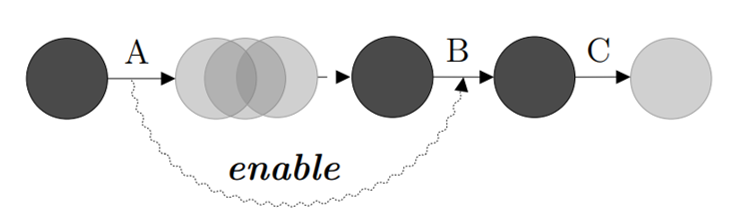
\includegraphics[width=0.8\textwidth]{Images/oppurtunity chain.png}
    \caption{An example of an oppurtunity chain, reproduced from \cite{madumal2020distal}, representing the causal relationship: ‘$A$ enables $B$ and $B$ causes $C$’. Here, the nodes represent states and $A$, $B$ and $C$ denote actions. The action $B$ is referred to as the distal action.}
    \label{fig:oppurtunity chain}
\end{figure}

\noindent These distal actions are identified from replay data collected during agent training using a recurrent neural network (RNN), and used in conjunction with the action influence explanation method proposed in \cite{madumal2020explainable}. The authors also replace the regression models used to learn the structural equations in the AIM with a decision tree model in order to provide decision boundaries as part of the explanation. In particular, the explanation given in Figure \ref{fig:action-influence} for the question `why not take action $A_b$' is extended to: `Because ally unit number $A_n$ is less than the optimal number 18, it is more desirable to do the action $A_m$ to enable the action attack $A_a$, as the goal is to have more Destroyed Units ($D_u$) and Destroyed buildings ($D_b$).' Here, $A_n = 18$ is the decision boundary learnt via the decision tree, and $A_a$ is the distal action learnt by the RNN.

Again, the explanation model is evaluated both using RL benchmarks domains and a human study investigating task prediction and explanation satisfaction in the simplified Starcraft II domain, yielding promising results compared to two baseline explanation models. However, the major disadvantage of both \cite{madumal2020distal} and \cite{madumal2020explainable} is that the methods are only applicable in situations where an action influence model can be defined. In particular, the causal relationships must be known a priori, and these must correspond to specific actions available to the agent. While causal discovery methods may be able to aid in defining causal relationships, the problem still remains to match these with corresponding actions. This limits the applicability of the approach. Indeed, the model has only been evaluated in the simple Starcraft II scenario, so further work would be needed to investigate whether the promising results of the human study translate to more complex problems. Additionally, the method requires data collected during agent training (thus falling into the `Training data' category in Figure \ref{fig:xrl_taxonomy}), meaning that the approach cannot be applied to already trained agents. 



\subsubsection{Causal state and temporal importance}

An alternative approach to local explanation generation for RL agents avoids the issue of matching actions to causal links by representing the action as a node itself in the causal graph. In \cite{wang2022causal}, the authors provide explanations for specific agent actions via a three-step process. 

First, they construct a temporal causal graph between states and actions, as exemplified in Figure \ref{fig:state-action-causal-graph}. The causal links between state variables are assumed to be known, and with regard to the state-action links, the authors assume a general case where all (endogenous) variables observed by the agent influence the action taken. 

\begin{figure}[htp]
    \centering
    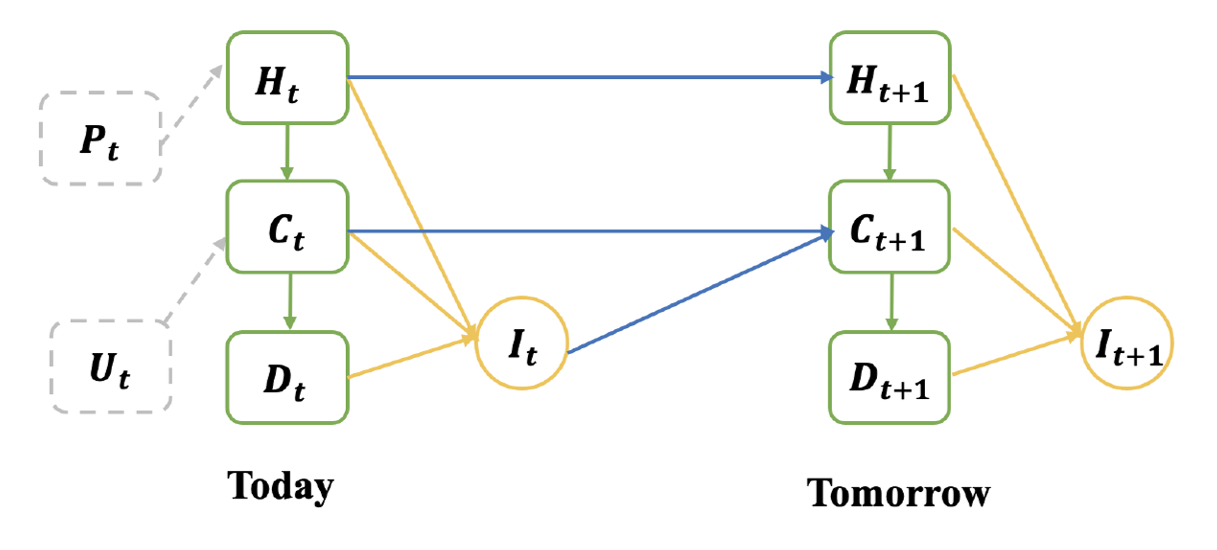
\includegraphics[width=0.8\textwidth]{Images/state-action-causal-graph.png}
    \caption{An example of a temporal causal diagram for a crop irrigation RL scenario, taken from \cite{wang2022causal}. Dashed and solid rectangles represent endogenous and exogenous state variables respectively, while circles denote actions. Such diagrams are used to define the causal links in an SCM in order to calculate the outcome of counterfactual instances.} 
    \label{fig:state-action-causal-graph}
\end{figure}

Next, a dataset of post-training episodes is collected by allowing a pre-trained DeepRL agent to interact with the environment of interest. This is used to approximate the structural equations associated with the causal graph via supervised learning, and the authors provide examples in which they used various techniques including linear regression and a neural network.

Finally, the influence of each state variable on a specific action is quantified via a counterfactual feature importance calculation. Specifically, suppose that at time $t$ we observe a state $\mathbf{S_t} = \mathbf{s_t} $ where $S_t^{(i)}$ denote individual state variables for some $i = 1,...,n$, and suppose that the action taken by the agent was $a_t$. Then the importance weighting for feature $S_t^{(i)}$ is calculated as:

\begin{align}
\label{eq: paper_weightings}
    w^{(i)}_t &= \frac{||(A_{t, S^{(i)}_t = s_t^{(i)} + \delta} | \mathbf{S_t = s_t}, A_t = a_t) - a_t ||}{\delta},  
\end{align}

\noindentwhere $|| . ||$ denotes a vector norm, and $\delta $ a small perturbation value chosen with regard to the application. Here, the $(A_{t, S^{(i)}_t = s_t^{(i)} + \delta} | S_t = s_t, A_t = a_t)$ term denotes the counterfactual outcome of $A_t$ if $S_t$ had been equal to $s_t + \delta$. The authors calculate the value of $w_t^{(i)}$ for each state variable, with higher values of $w_t^{(i)}$ indicating that the corresponding feature had a greater influence on the choice of the action $a_t$. 

The feature weightings $w_t^{(i)}$ can be calculated for each time step within an episode to produce a temporal graph indicating how feature importance values vary as the scenario progresses. An example of such a graph is shown in Figure \ref{fig:state-temporal-importance}.

\begin{figure}[ht]
    \centering
    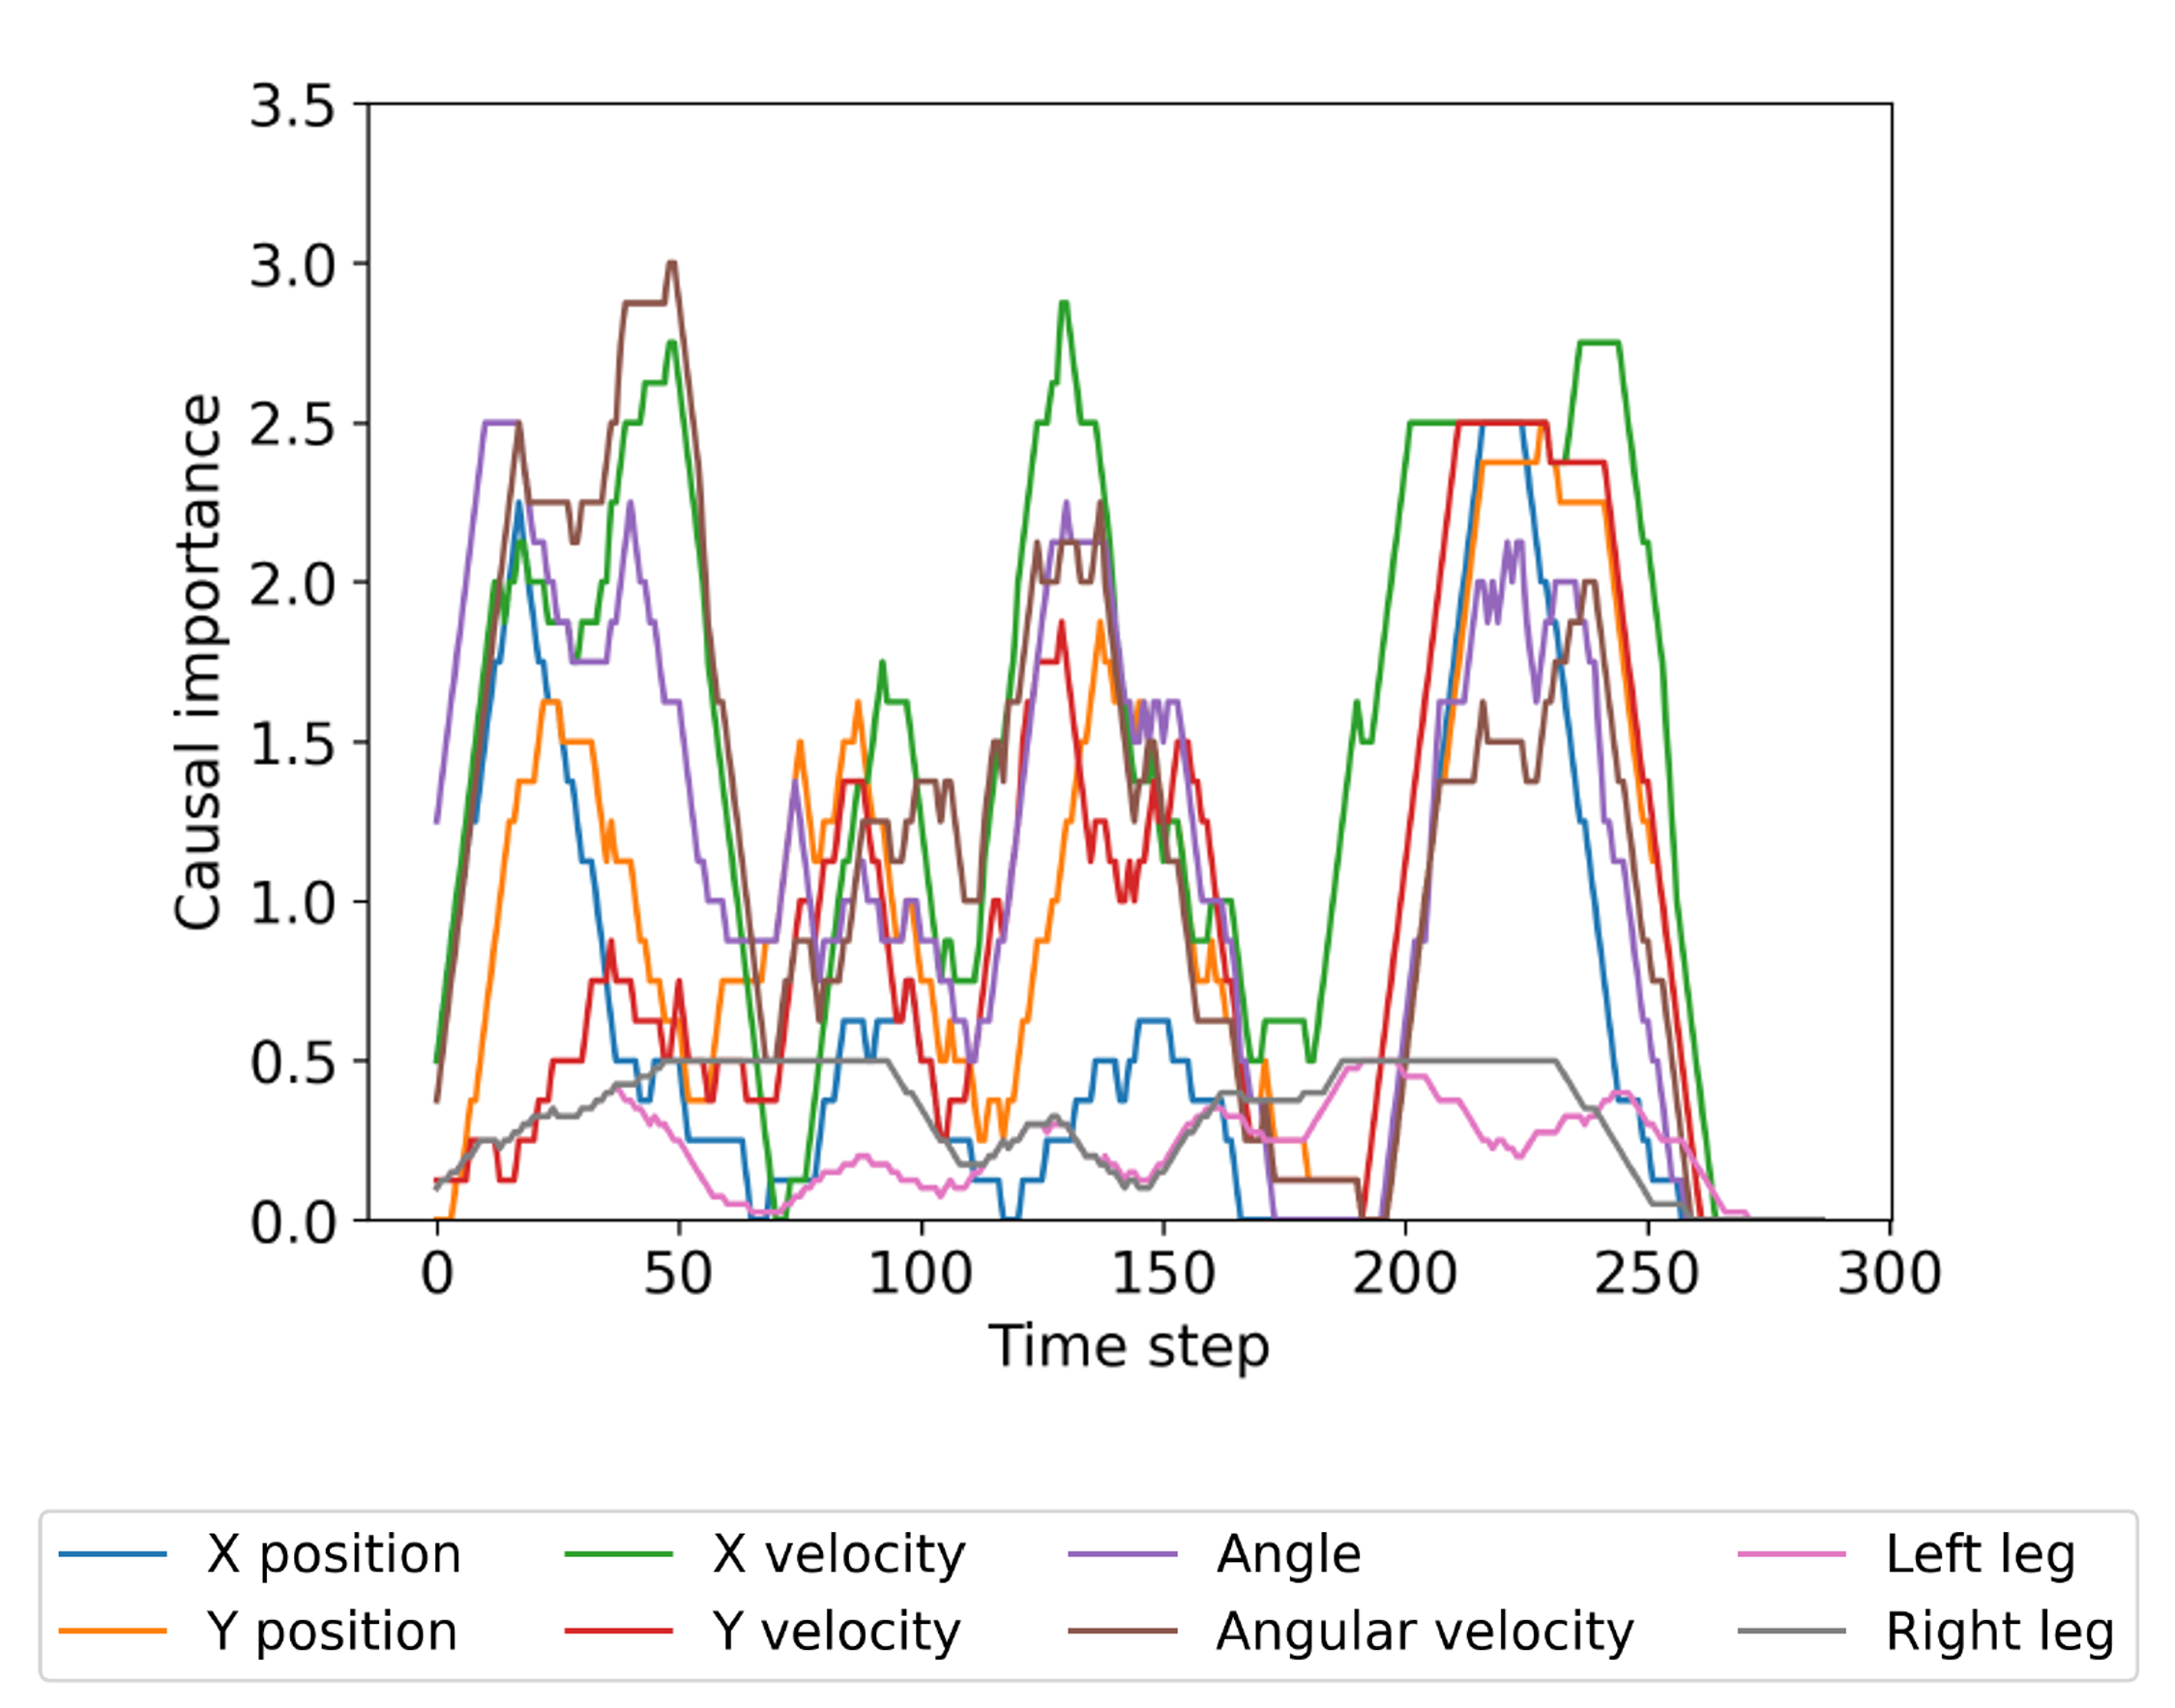
\includegraphics[width=0.8\textwidth]{Images/state-temporal-importance.png}
    \caption{An example of a temporal importance graph for an episode of the lunar lander scenario, taken from \cite{wang2022causal}. Here the aim of the agent is to successfully land a rocket on a landing pad whilst conserving fuel, and the available actions are to fire the main, left, or right engine, or to do nothing. The observed features are given in the legend, and their causal importance calculated using Equation (\ref{eq: paper_weightings}) for each time step. } 
    \label{fig:state-temporal-importance}
\end{figure}

The main advantage of this method over the associational techniques discussed in Section 3.2 is that associational models lack the capability to perform in local counterfactual reasoning \cite{wang2022causal}. By contrast, the causal method in \cite{wang2022causal} uses counterfactual reasoning to recover the environment at the current state and approximate the response of the system when one of the state features is changed. Hence, causal importance has the capacity to derive a greater depth of insight into the impact of the change in value. In particular, in the case where a state variable, $V^{(i)}$ is a causal parent of other features, the method is able to capture not only the direct effect of altering $V^{(i)}$ on the action, but also its effect through its causal children. For example, referring to Figure \ref{fig:state-action-causal-graph}, through the calculation of counterfactuals, the causal method is able to capture the effect of varying $C_t$ through two causal chains; $C_t \rightarrow I_t$  and $C_t \rightarrow D_t \rightarrow I_t$.

Unfortunately, this paper omits many important calculation details, such as the meaning of subtracting action values when in many of their examples, the action is a categorical variable. For instance, in the lunar lander scenario, where the aim of the RL agent is to land a rocket on a landing pad, the available actions are `fire main engine', `fire left engine', `fire right engine' and `do nothing'. These have no obvious concept of subtraction. Further, the authors don't specify which vector norm is used in their calculations, nor give specific insight into their choice of perturbation value $\delta$. The examples presented in \cite{wang2022causal} are also very simplistic (lunar lander, blackjack and the toy crop irrigation problem illustrated in Figure \ref{fig:state-action-causal-graph}. 

In this report, I aim to improve on the weighting calculation method for the specific case of a cybersimulation problem, and specify the ommitted details. Additionally, I  create a temporal importance diagram similar to Figure \ref{fig:state-temporal-importance} for a cyber defence episode, and use this to give insights into how the state variables influence the decisions of a trained PPO agent. The authors of \cite{wang2022causal} extend their work by defining an additional weighting calculation method for value-based reinforcement learning, and demonstrating how the causal chain can be cascaded to determine the effect of past variables on the action choice. However, this is beyond the scope of this report. 

\subsection{Limitations in XRL studies}

While reviewing papers surrounding XRL, several recurrent limitations arose, notably the prevalence of specific "toy examples" with little scalability and the lack of consistent evaluation metrics or sufficient user testing. The forthcoming subsection investigates these shortfalls in greater detail. 

\subsubsection{Scalability and use of specific examples}

All of the papers encountered while performing this review presented essentially `toy' applications; for the majority of cases games such as Starcraft \cite{madumal2020explainable}, Blackjack \cite{wang2022causal}, Frogger \cite{ehsan2019automated} and Space invaders \cite{greydanus2018visualizing}. These generally feature relatively small state and action spaces, and simple system dynamics. This trend is consistent with that found in \cite{wells2021explainable}, a comprehensive review of 25 XRL studies, in which 16 were found to either focus on agents trained for video game scenarios or test their methods on video game problems. 

This bound in scope is generally to avoid problems associated with combinatory explosions, where a growth of state and action spaces corresponds to a huge increase in the number of possible state-action pairs. However, this limits the scalability of such approaches, resulting in fewer cases in which XRL methods can be meaningfully applied. This seems particularly true of causal explanation generation mechanisms, as exemplified in  Section 3.3, where all reviewed methods require a causal diagram between states (\cite{madumal2020distal}, \cite{madumal2020explainable}, \cite{wang2022causal}). 


\subsubsection{User testing and evaluation metrics}

Whilst the majority of studies encountered for this review motivated their work by citing sources from psychology, many of the techniques presented did not feature a human study, and when these were present, they were often vague on key details such as where the participants were recruited from and whether they were knowledgeable about machine learning. Further, varying numbers of participants have been used in such experiments, ranging from just three experts used in \cite{wang2018dqnviz} to 191 in \cite{huang2019enabling}, however even the largest are still very small studies when compared to other fields \cite{wells2021explainable}. The lack of user testing observed in this review aligns with the findings in the Miller et. al review of XAI research in general \cite{miller2017explainable}. As the purpose of XRL is to extract human-understandable reasoning from complex models, more thorough and consistent human-focussed evaluation is needed to ensure the validity of XRL methods.

Even aside from user testing, there do not yet exist agreed metrics or benchmarks by which to evaluate XRL techniques. This is due in part to the lack of a consistent definition of what constitutes explainability, as discussed in Section 3.1, and also to the varying target audiences between studies. However, without benchmarks and evaluation metrics it is very difficult to compare methods presented in different papers and so their development is of great importance to the field \cite{ehsan2019automated}.


%--------------------------------------------------------


\pagebreak

\section{YAWNING TITAN}
% Introduce and explain YT, formulate the problem and lay out the aims
In this section, I introduce the cybersimulator, YAWNING TITAN, used in this paper, and define the parameters for the reinforcement learning scenario.

YAWNING TITAN (henceforth abbreviated YT)  is an abstract, graph-based cybersecurity simulator with a game-style format, built to enable the development of autonomous cyber defence agents \cite{YT}. In particular, the package allows the user to construct a connected network, upon which a probabilistic red agent performs malicious actions. In this network, the nodes represent computing devices within a computer network, and the edges connections between these devices. The task of the user is to train (or play as, via the keyboard agent capability) a blue agent, whose aim is to defend the network. One of the main design principles behind YT is flexibility, and as such the ‘winning criteria’, reward function and actions available to either agent are highly configurable, to reflect a variety of cyber defence scenarios such as intrusion response (where the aim is to remove an intruder from the network as quickly as possible) and crown jewels defence (where the attacker is aiming for a specific, high value target). A stochastic attacker was chosen rather than a deterministic one to ensure a diversity in its behaviour across training and evaluation.


YT is OpenAI compatible, enabling seamless experimentation with open source RL libraries such as Stable Baselines3. It also features a built in GUI for easy visualisation and alteration of the configuration file. In particular, the various aims, actions and game rules are all configurable. Further, one can easily create gifs of an episode, enabling the user to observe the agent's decisions and progress throughout the episode.  

We set up the environment and reinforcement learning scenario as follows. 

\subsection{Network initialisation and game setup}

Each YT scenario consists of two parts; a network and a 'game mode'. The network takes the form of an undirected graph $G = (V,E)$, where $V$ denotes a set of nodes, and $E$ the set of edges between them. Each node within the YT network has two main attributes; a vulnerability score, $V$, and compromised status, $C$. The vulnerability score is an integer $V \in [0,1]$, and can be thought of as an abstract indicator of the relative number of vulnerabilities a specific device has. This attribute is incorporated into the probability that an attack on the node will succeed, allowing for variability in the ease of compromising nodes. The compromised status is a binary value indicating whether the node is currently occupied by the red agent ($c=1$), or not ($c=0$). At the beginning of each episode, all nodes are uncompromised.

The YT network also consists of `special' node types. In particular, the graph must contain at least one entry node, which acts as the red agent's preliminary target and route into the network. This can be interpreted as an externally facing device which is the initial focus of the attacker. Nodes in the network can also be configured to the `high value' type. This is designed to represent cases in which the attacker has specific targets within the network.

The YT 'game mode' is a configuration file specifying the parameters of the simulation environment, such as the reward function, the action spaces of both the defending and attacking agents, and the maximum number of time steps in an episode. This file also specifies the objective of the red agent. This could be total compromise of the network, which has similarities to the stagnating phase of a ransomware attack, where the attackers aim is to gain control of as many assets as possible \cite{collyer2022acd}. Alternatively, one can consider the case where the red agent's goal is to compromise a specific high value node, which emulates the real life scenario in which classified information that an attacker is trying to gain access to is stored on a specific device. In this research, we will consider the latter objective. 

\begin{figure}[htp]
    \centering
    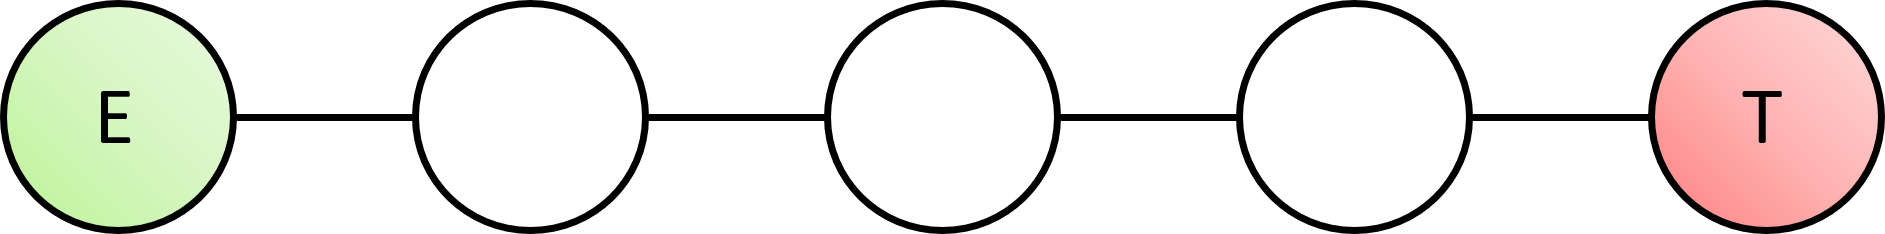
\includegraphics[width=0.8\textwidth]{Images/linear_5_PC.png}
    \caption{The linear 5 PC network. The green node represents the entry point, and the red indicates the high value target.}
    \label{fig:linear_5PC_diagram}
\end{figure}

For the purpose of this work, we will consider a linear, 5 node network as shown in Figure \ref{fig:linear_5PC_diagram}. The entry and high value target nodes will be situated at either end of the network, and we will refer to the nodes as $1,2,3,4$ and 5 from left to right. This configuration has been chosen to create the simplest possible structure for considering causality, whilst allowing enough distance between the entry and target for episode diversity. This is because the causal graph complexity grows rapidly with the number of nodes, but distance is needed so that episodes last long enough to facilitate proper training of the blue agent; if entry and target are too close, the red agent will likely win regardless of the actions taken by the blue agent.


\noindent We will denote the compromised status and vulnerability for each node $i$ as $C^{(i)}$ and $V^{(i)}$ respectively. Each episode begins with $C^{(i)} = 0$, $V^{(i)} = 0.8$ for all $i = 1,...,5$. Game-play evolves with each agent taking it in turns to act. Specifically, the order of execution is as follows:
\begin{enumerate}
    \item Blue agent receives an observation of the state space.
    \item Red agent acts.
    \item Environment checks whether red agent has won.
    \item Blue agent acts.
    \item Reward for the time step is returned to the blue agent.
    
\end{enumerate}

The aim of the red agent is to compromise the high value node 5, in which event the episode is terminated. The maximum number of time steps for each episode is set to 30. The aim of the blue agent is to reach this maximum duration.

\subsection{Blue agent configuration}

\subsubsection{Action space}

The actions available to the blue agent at each time step are given in Table \ref{tab:blue_actions}. Skip is a global action, whilst Reduce and Patch are applied to a specific node, giving a total of 11 possible actions.

\begin{table}[h!]
    \centering
    \small
    \begin{tabular}{ | m{0.2\textwidth} | m{0.6\textwidth}|} 
      \hline
       \textbf{Action} & \textbf{Description} \\ 
      \hline
        Reduce$_i$ & Reduce the vulnerability of node $i$ by 0.2. \\ 
      \hline
        Patch$_i$ &  Remove red compromise from node $i$. \\ 
      \hline
        Skip &  No change is made in this time step. \\ 
      \hline
      
    \end{tabular}
    \caption{The actions available to the blue agent.}
    \label{tab:blue_actions}
\end{table}

This action space has been chosen to permit both proactive (reduce) and reactive (patch) responses whilst keeping the game setup relatively simple. The reduce value of 0.2 was selected to offer the agent a method to reduce node vulnerability by a significant degree, whilst at the same time imposing limitations on the capacity to generate near invulnerable hosts and exploit the simulation. Note that node vulnerability need not be further bounded due to the attack success probability configuration explained in Section 4.3; a vulnerability score of 0 does not correspond to a completely invulnerable node. A skip action is also permitted since the actions have associated costs, as defined in Section 4.4.

\subsubsection{Observation space}
At each time step, the blue agent observes the current state of the environment in the form of a $9 \times 5$ matrix. An example of such an observation is shown in Figure \ref{fig:example_obs}.

\begin{figure}[htp]
    \centering
    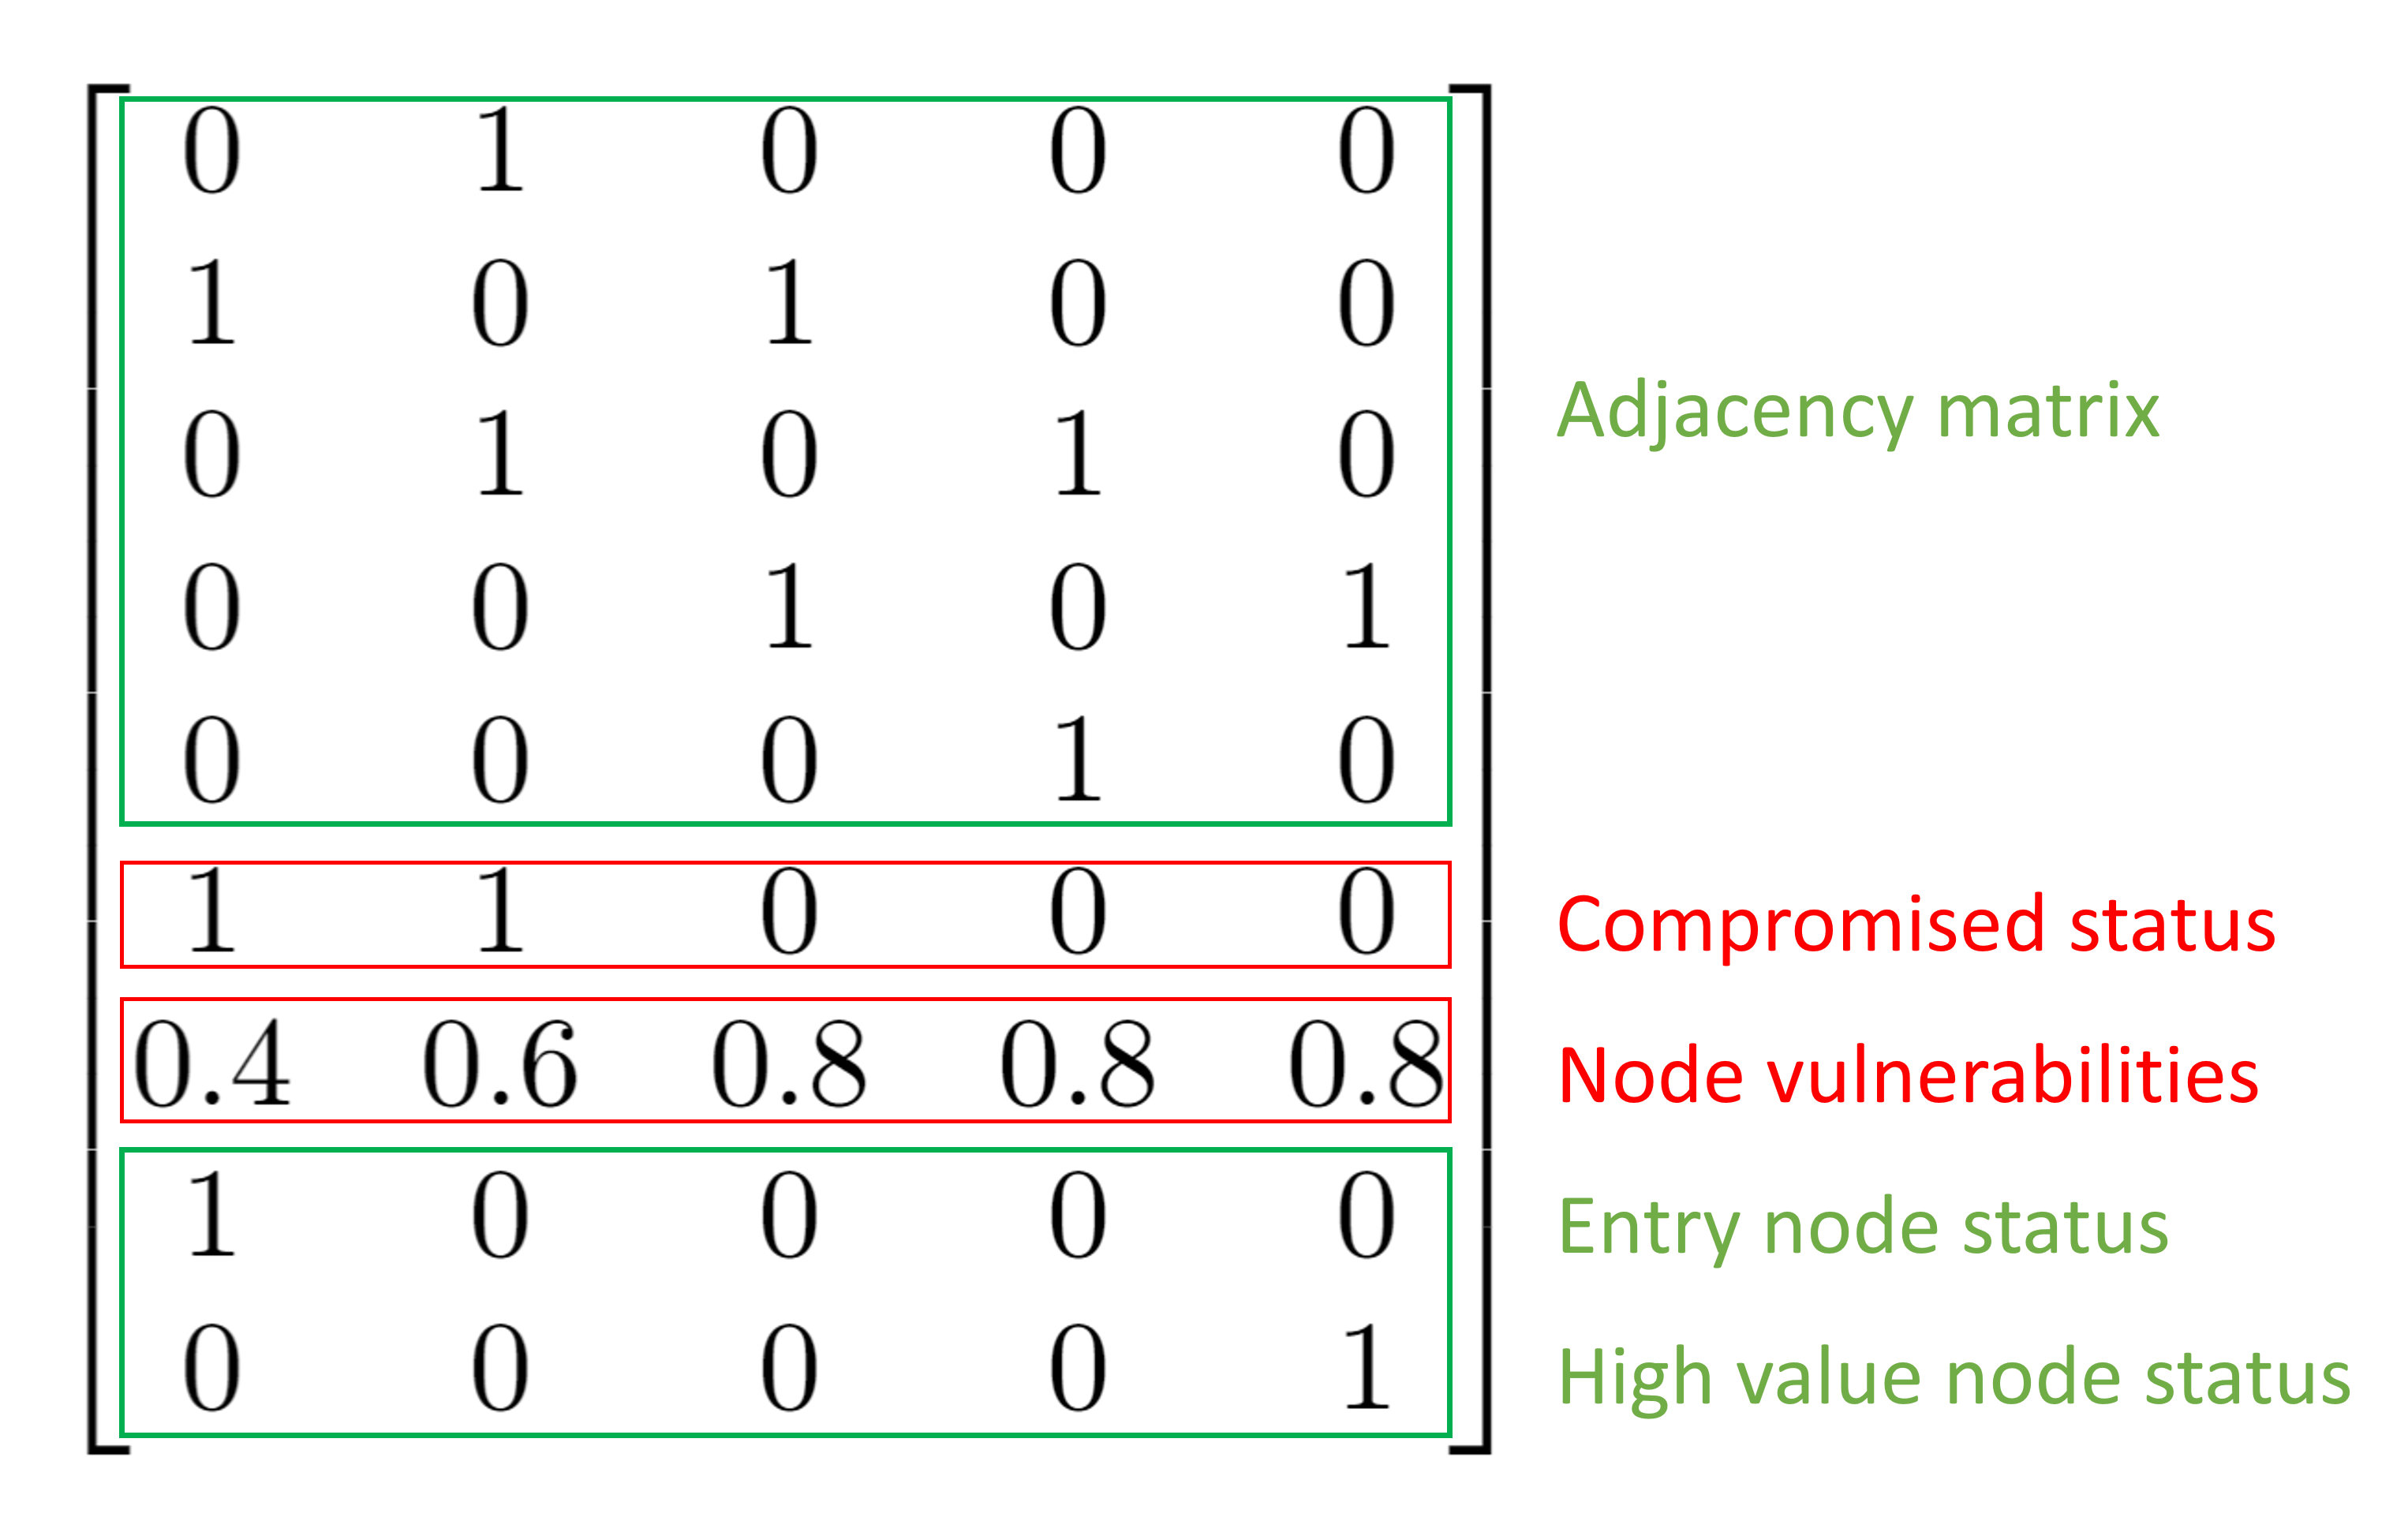
\includegraphics[width=0.6\textwidth]{Images/Example_obs.png}
    \caption{An example observation matrix. Red indicates variables which change over the episode, whilst green indicates static variables. }
    \label{fig:example_obs}
\end{figure}

In particular, the blue agent observes the node connections in the form of an adjacency matrix ($5 \times 5$ matrix of binary values where a 1 indicates an edge is present between the nodes indexed by the column and row) along with the compromised status of each node, the current node vulnerabilities and special node types (entry or high value). The adjacency matrix and special node types remain constant throughout each episode, while the compromised status and node vulnerabilities are variable. 


\subsection{Red agent configuration}

The red agent is entirely probabilistic, and on its turn, either attacks the next available node or does nothing. There are two available attack types; zero-day or a basic attack. A zero-day attack is a guaranteed node compromise regardless of the node's vulnerability score. The red agent begins each episode with a single zero-day attack and gains another every 5 time steps. These zero-day attacks are used as soon as they are available, and are designed to ensure that the red agent can make progress in the network even if the blue agent has significantly reduced node vulnerabilities. 

If a zero-day attack is not available, a basic attack is deployed with probability 0.8, else the attacker does nothing for a turn. The probability of success of a basic attack is based on the target node vulnerability and the red agent's skill; a value $r \in [0,1]$ chosen prior to the episode. The mechanism which determines whether an attack was successful is inbuilt in YT and was constructed so that the `likelihood for the
red agent to compromise a node increases proportionately with the skill of the agent and decreases proportionately with the defence of the node' \cite{collyer2022acd}. In particular, suppose node, $i$, is being attacked and has vulnerability $v^{(i)}$. We define the attack strength, $s$, by:
\begin{align}
    s = \frac{r^2}{r + (1-v^{(i)})}.
\end{align}

Following the calculation of the attack strength, a threshold $t$ is drawn from a uniform distribution, $t \sim \mathcal{U}(0,1)$. The attack is successful if $s > t$. In particular, the target node is compromised with probability $s$.   

As the probability of a node compromise impacts the ability of the red agent to make progress in the network, the choice of $r$ is important in ensuring a balanced game scenario. In particular, if the value of $r$ is too high, then the red agent will dominate the scenario and prevent the blue agent from effectively training. A value of $r$ too low makes the game `too easy' for the blue agent, again hindering effective training as the red agent can make little progress in the network. From Figure \ref{fig:attack strength} we can also see that the lower the value of $r$, the smaller the advantage gained when the vulnerability of a node is reduced, reducing the ability of the blue agent to proactively defend nodes. 

To make this choice, the value of $r$ was experimentally varied, while all other YT parameters remained fixed. A plot of the 5 attack strengths tested is shown in Figure \ref{fig:attack strength}. A PPO agent was trained for 100,000 episodes for each value of $r$, and the training curves with respect to average reward and average episode length were inspected. From these a value of $r=0.8$ was chosen for this work, resulting in an attack success probability ranging between 0.36 and 0.80.


\begin{figure}[htp]
    \centering
    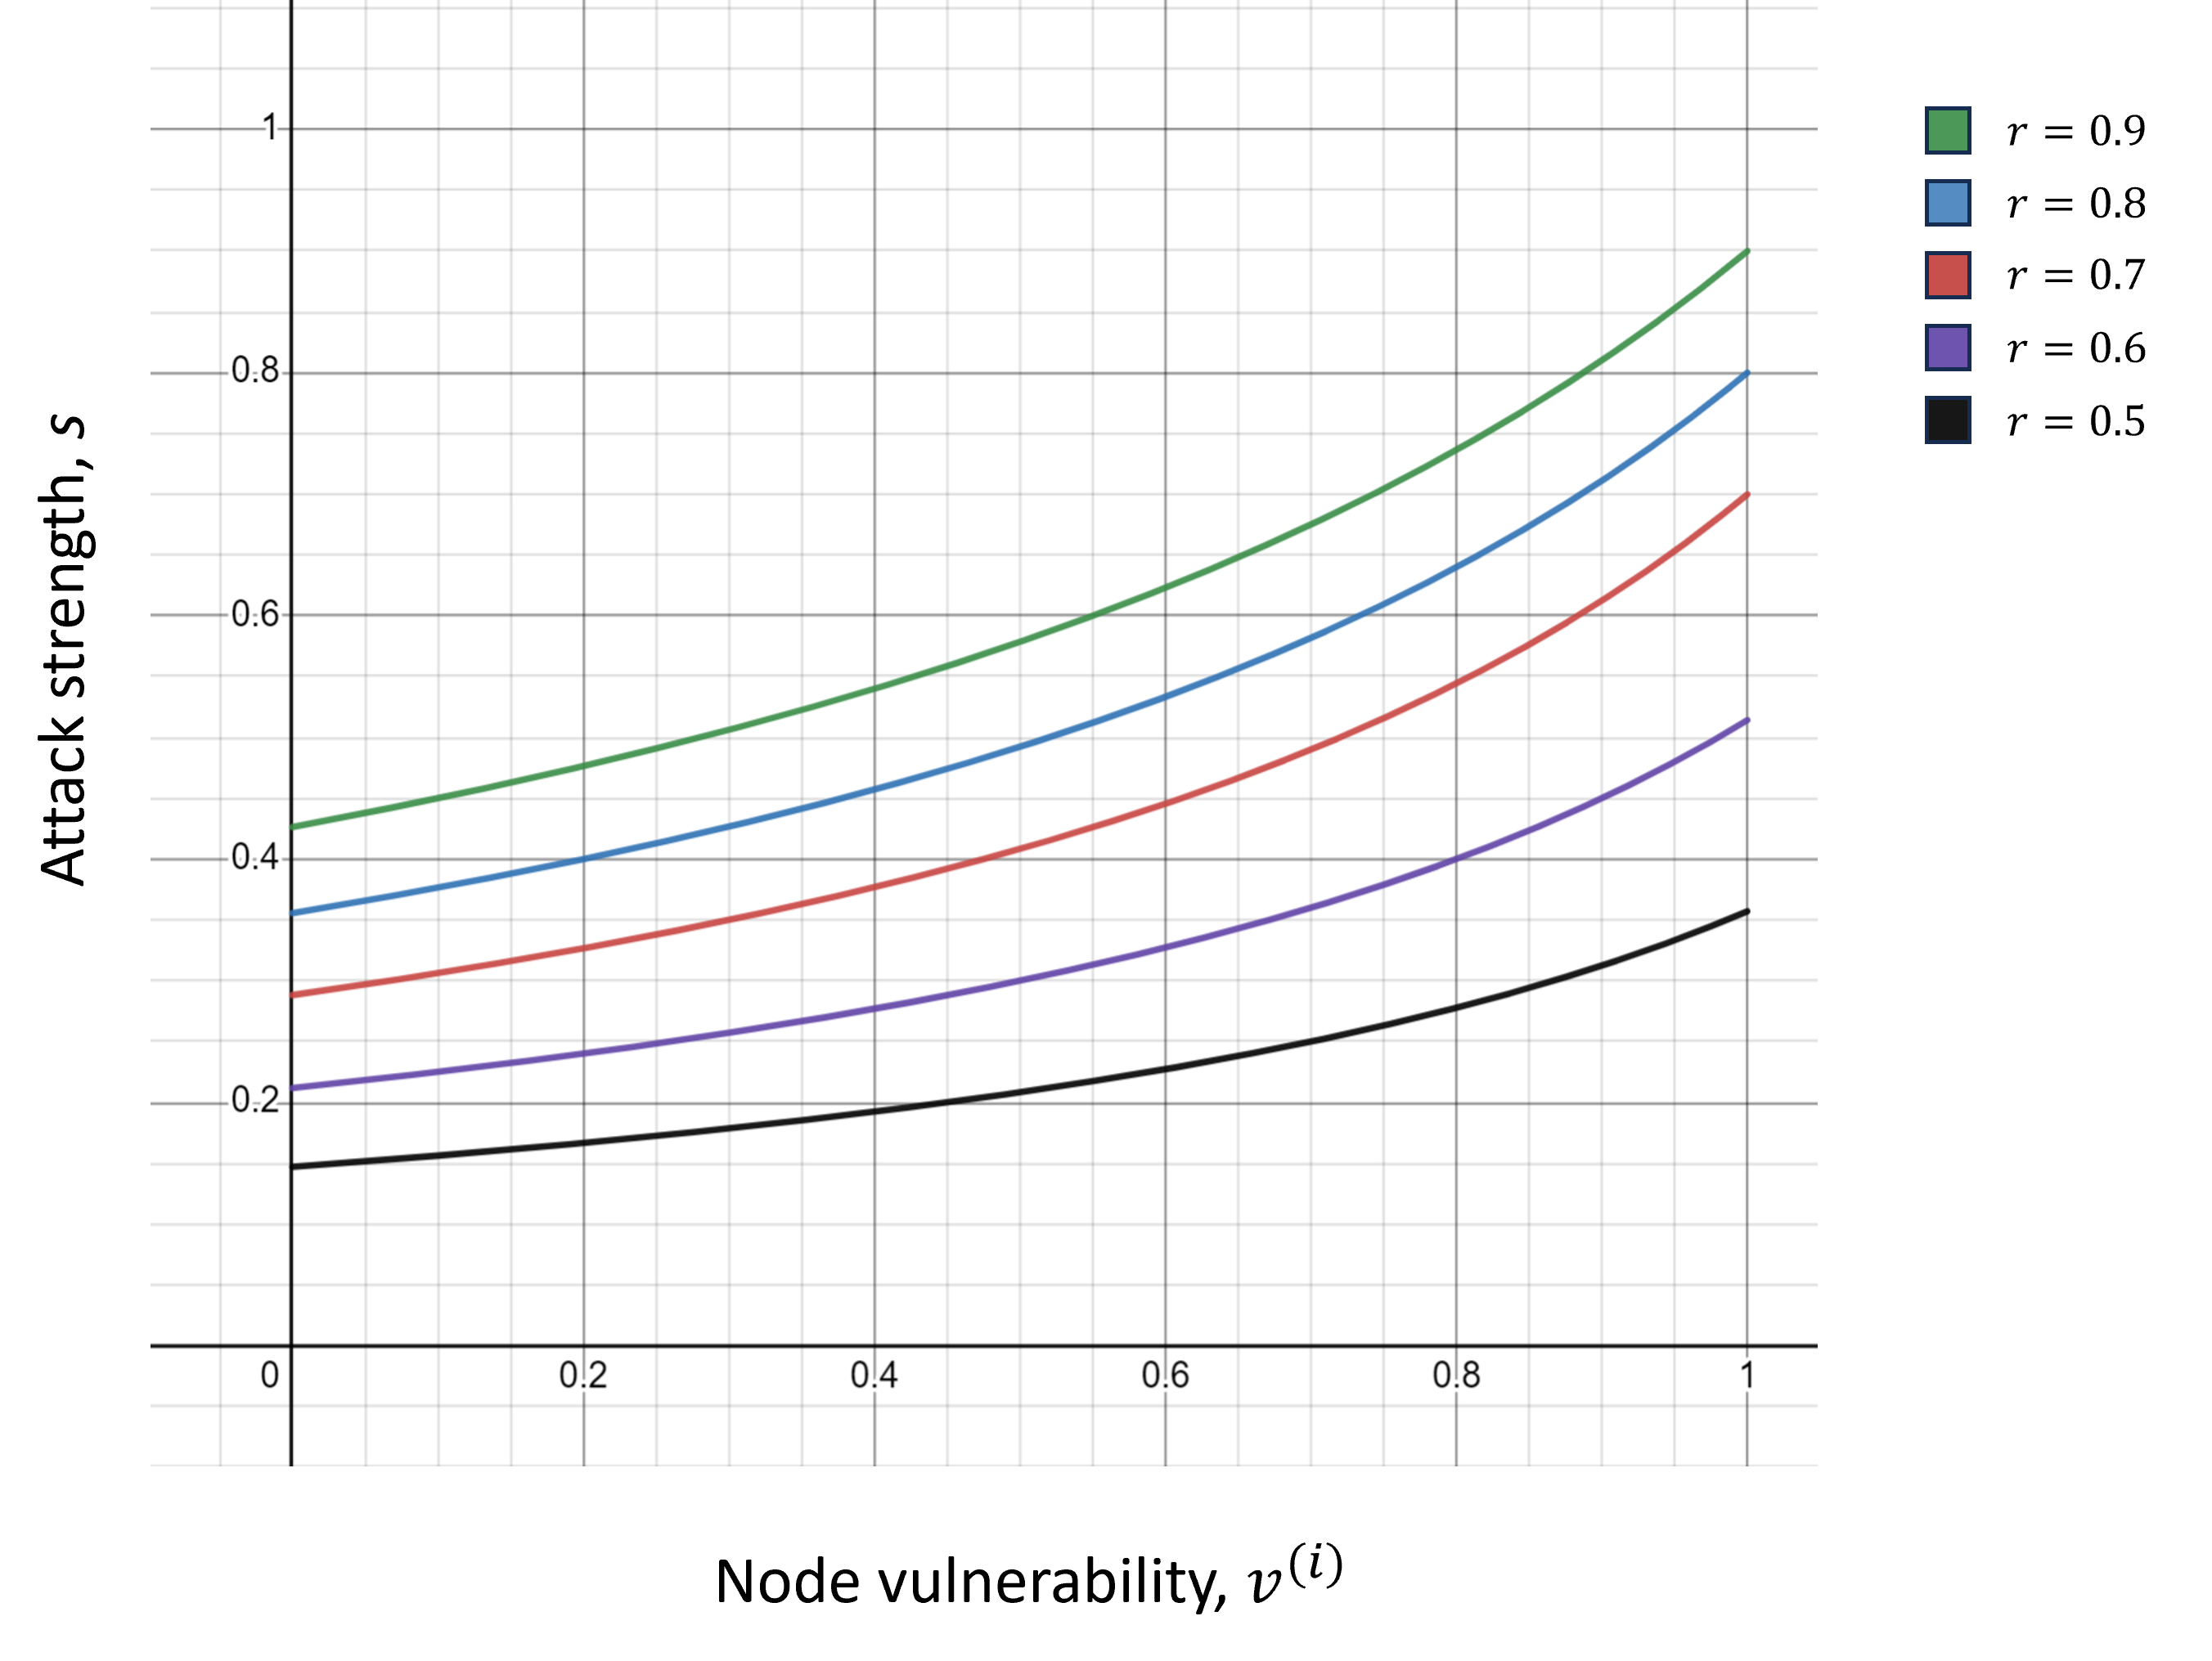
\includegraphics[width=0.6\textwidth]{Images/attack_strength.png}
    \caption{A plot of $s = \frac{r^2}{r + (1 - v^{(i)})}$ for different values of $r$. It was found experimentally that choosing $r = 0.8$ creates the best balance between the ability of the red agent to make progress in the network and the ability of the blue agent to successfuly defend nodes. }
    \label{fig:attack strength}
\end{figure}


\subsection{Reward function}
The rewards gained by the agent at time step $t$ ($t$ = 0,...,29) are summarised in Table \ref{tab:rewards}, and make up the \textit{standard rewards} provided in YT \cite{YT}. The first two entries give the terminal reward, depending on whether the red or blue agent was successful.

\begin{table}[h!]
    \centering
    \small
    \begin{tabular}{| m{0.18\textwidth} | m{0.55\textwidth} | m{0.18\textwidth}|} 
      \hline
       \textbf{Reward} & \textbf{Trigger} & \textbf{Value} \\ 
      \hline
        Blue loss & $C^{(5)}_t = 1$   & $-100(1-t/30)$ \\ 
      \hline
        Blue win & $C^{(5)}_{30} = 0$ & 100 \\ 
      \hline 
        Patch cost & $A_t= Patch_i$ for any $i = 1,...,5$ & -1 \\ 
      \hline
        Vulnerability reduction cost & $A_t= Reduce_i$ for any $i = 1,...,5$ & -0.5 \\ 
      \hline
        No action reward & $A_t= Skip$  & 0.5 \\
      \hline
        Unnecessary patch penalty & $A_t = Patch_i$ when $C^{(i)}_t = 0$ for any $i = 1,...,5$ & -3 \\       %\hline
 %       $C^{(i)}_t = 0$ when $C^{(i)}_{t-1} = 1$ for any $i = 1,...,5$ & $e^{-0.004p}$ \\ 
%      \hline  
        %$V^{(i)}_t < V^{(i)}_{t-1}$ when $C^{(i)}_{t-1} = 1$ %for any $i = 1,...,5$ & $4(V^{(i)}_t - V^{(i)}_{t-1})$ %\\
      \hline
     
    \end{tabular}
    \caption{The rewards gained from the environment in time step $t$, $t = 0,...,29$. 
    %Here $p$ denotes the proportion of nodes occupied by the red agent at time $t-1$.
    }
    \label{tab:rewards}
\end{table}


\noindent The value of the penalty for blue loss in Table \ref{tab:rewards} illustrates how negative rewards are reduced for closer fails, which was implemented to allow smoother training. The action costs are defined within the YT code and the authors claim that these are designed to mimic real-world scenarios in which defensive actions would likely have different costs and timeframes \cite{collyer2022acd}. A small reward is given when the blue agent does nothing to discourage unnecessary actions and patching uncompromised nodes also yields a punishment. 

%A reward proportional to the number of compromised nodes is given when the blue agent successfully patches a node  and reducing the vulnerability of a node yields a reward proportional to the reduction to promote positive actions in the inital stages of training. 


\pagebreak

\section{Method}
In this section, I present the method used to quantify the temporal importance of each state variable on the action taken by the RL learner. In particular, following the training of the RL agent, feature importance is derived via two steps; first we learn the structural equations in the underlying causal model, then the importance weightings are calculated via counterfactual interventions. These weightings facilitate explanations of agent actions by enabling a comparison between the impact each feature of the observation space had on the agent's decisions.

\subsection{Agent training}
The reinforcement learner to be studied was trained using the Stable Baselines3 implementation of PPO \cite{stable-baselines3}, for 200,000 episodes. After each episode, the training environment was reset to the initial state specified in Section 4. The metrics tracked to evaluate training were episode length, average reward and loss. The training duration of 200,000 episodes was chosen as it proves sufficient for these metrics to plateau. 



\subsection{Causal structure}

\subsubsection{Causal diagram}
In order to calculate causal feature importance, we assume the temporal causal model given in Figure \ref{fig: YT causal graph}, which has been constructed by inspection of the environment. Note that constant features observed by the agent, node connections and special node types, are not shown in this network. This is because, as these observations do not change throughout the training, we assume them as a part of the environment and presume that their influence on the action taken remains constant. Furthermore, the influence of the adjacency matrix of the YT network is encoded implicitly in Figure \ref{fig: YT causal graph} via the causal relations between node attributes. For example we assume a causal connection between $C_t^{(1)}$ and $C_t^{(2)}$ since node 2 cannot be compromised if node 1 hasn't been compromised due to the network topology. Much of Sections 5.2 and 5.3 are inspired by the method presented in \cite{wang2022causal}, with alterations made to suit the YT scenario.

\begin{figure}[htp]
    \centering
    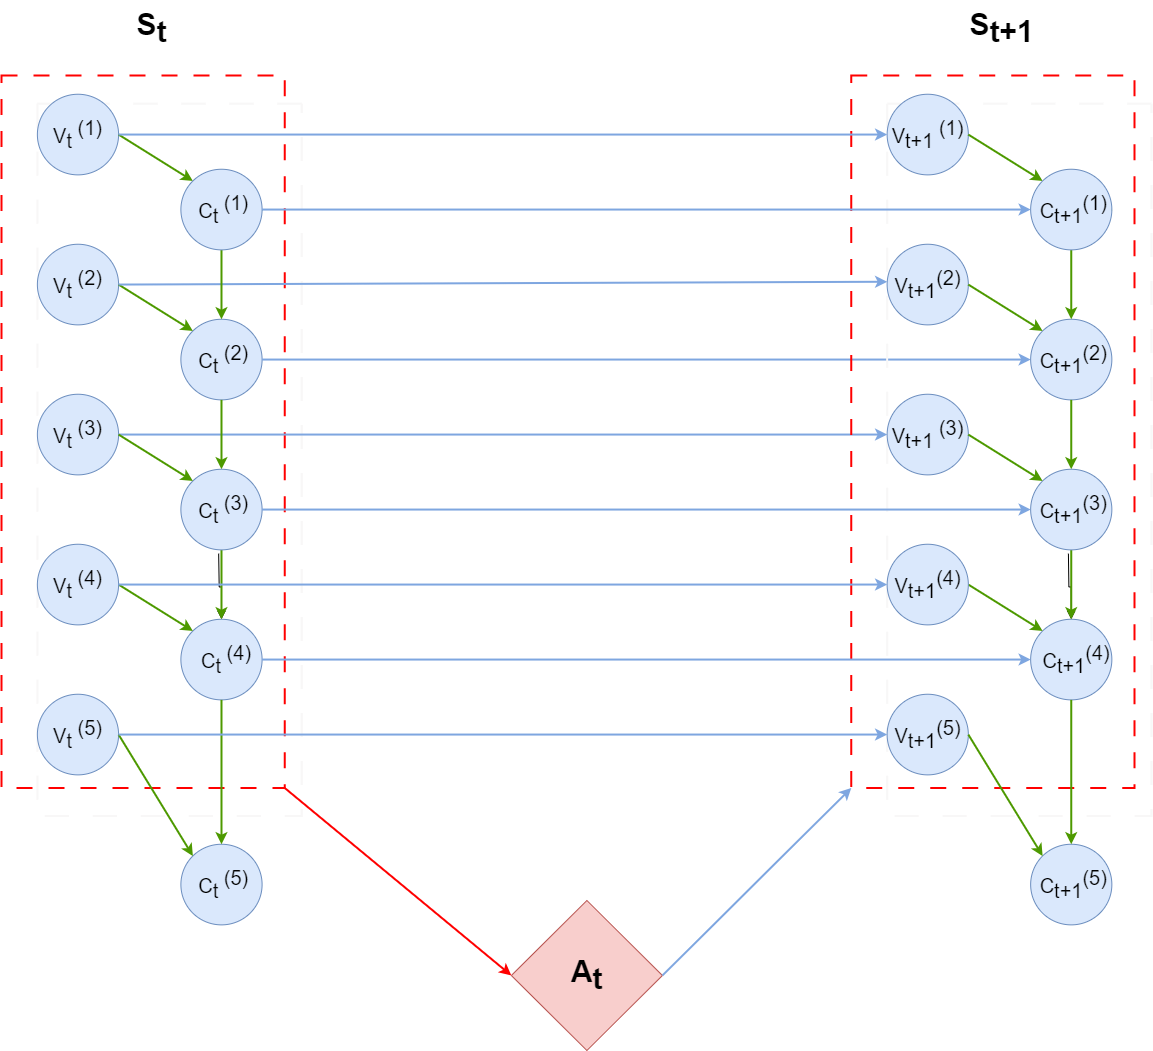
\includegraphics[width=0.9\textwidth]{Images/YT Causal Diagram.drawio.png}
    \caption{The assumed causal model for the YT environment, linking states to actions over time steps $t= 0,...,29$. The red boxes indicate that arrows should be present from or to every node inside, however these have been omitted for simplicity.}
    \label{fig: YT causal graph}
\end{figure}

We can partition the causal relations in Figure \ref{fig: YT causal graph} into 3 types, given in Table \ref{tab:causal_relations}. 

%\pagebreak

\begin{table}[h!]
    \centering
    \small
    \begin{tabular}{ | m{0.22\textwidth} | m{0.2\textwidth}| m{0.5\textwidth}|} 
      \hline
       \textbf{Type} & \textbf{Arrow colour in Figure \ref{fig: YT causal graph}} & \textbf{Explanation}\\ 
      \hline
         Intra-state & Green & Relations specified by the underlying causal mechanism \\ 
      \hline
         Transition-defined & Blue & Relations representing the relationship between states across time steps. \\ 
      \hline
         Policy-defined & Red & Relations expressing how states affect the action as defined by the policy of the RL agent.\\ 
      \hline
     
    \end{tabular}
    \caption{The three types of causal relation in a state-action causal graph, with the corresponding colour of arrow in Figure \ref{fig: YT causal graph}.}
    \label{tab:causal_relations}
\end{table}

\noindent For the purpose of this work, we assume a general case where all observable state features have a causal influence on the action. Hence in Figure \ref{fig: YT causal graph}, policy-defined relations are shown between all variables in $S_t$ and the action, $A_t$, with the exception of state feature $C_t^{(5)}$. This exclusion is because $C_t^{(5)}$ is a terminal state. In particular, if $C_t^{(5)} = 1$, then the episode terminates at time step $t$ and so there is no such $A_t$, nor $S_{t+1}$. We further assume that Figure \ref{fig: YT causal graph} captures all transition-defined and intra-state relationships between the given variables in the YT scenario.

\subsubsection{Structural equations}

The problem remains to learn the structural functions between each vertex in Figure \ref{fig: YT causal graph} and its parents. This amounts to learning functions of the form:

\begin{align}
     A_t &= f_a\left(C_t^{(1)}, C_t^{(2)}, C_t^{(3)}, C_t^{(4)}, V_t^{(1)}, V_t^{(2)}, V_t^{(3)}, V_t^{(4)}, V_t^{(5)}\right) + U_a 
     \label{eq: A structural equation}\\
\label{eq: C structural equation}  
    C_t^{(i)} &= f_{C^{(i)}}\left(V_t^{(i)}, A_{t-1}, C_{t-1}^{(i)}, C_{t}^{(i-1)}\right) + U_{C^{(i)}} \textnormal{ for i = 2,3,4 and } \\
\label{eq: C1 structual equation}
    C_t^{(1)} &= f_{C^{(1)}}\left(V_t^{(1)}, A_{t-1}, C_{t-1}^{(1)}, \right) + U_{C^{(1)}} \\
\label{eq: V structural equation}
    V_t^{(i)} &= f_{V^{(i)}}\left(V_{t-1}^{(i)}, A_{t-1}\right),   
\end{align}

\noindent where $t = 0,...,29$, $C_0^{(i)} = 0$, $V_0^{(i)} = 0.8$ and $i = 1,..,5$. Here, the $U_-$ variables denote unobserved exogenous variables in the form of an additive noise assumption widely used in causal discovery literature \cite{wang2022causal}.  Intuitively, for our application, the variables $U_-$ capture the stochasticity of the PPO policy in the policy-defined relations, and the stochasticity of the environment caused by the red agent in the transition-defined relations. 


The Equations (\ref{eq: A structural equation}), (\ref{eq: C structural equation}) and (\ref{eq: C1 structual equation}) are approximated via logistic regression models, trained using interaction data between the agent and environment. Due to the efficacy of the policy learnt by the trained agent, when running evaluation episodes it was found that there was rarely a case where more than one node was compromised. Thus, a dataset constructed by simply running evaluation episodes, as recommended for learning the structural equations in \cite{wang2022causal}, is insufficient in this case. In particular, the regression models will not be able to accurately predict the counterfactual outcomes when multiple nodes are compromised if such instances have not occurred in their training data.

Thus instead, the dataset was constructed by first sampling 10,000 random states from the state space defined in Section 4, and then collecting the agent's predicted action starting from each of these states. The YT environment was then stepped to obtain the resulting state from the chosen action, resulting in a dataset of entries of the form $(S_t, A_t, S_{t+1})$, where $S_t$ and $S_{t+1}$ represent the values of the state variables before and after the predicted action $A_t$. The regression models were trained on a random sample of 90\% of the data instances and evaluated on the remainder. All achieved above 95\% prediction accuracy. 


The equations (\ref{eq: V structural equation}) do not need to be learnt, as the nature of the YT environment means that $V_t^{(i)}$ is determined completely by $V_{t-1}^{(i)}$ and $A_{t-1}$. Specifically, we can write:
\begin{align}
    V_t^{(i)} = V_{t-1}^{(i)} - 0.2 \times \mathds{1}(A_{t-1} = \textnormal{`Reduce the vulnerability of node } i \textnormal{'.}),
\end{align}
\noindent where $\mathds{1}$ denotes the indicator function; the vulnerability of a node only changes if an action is taken by the agent to reduce it. In particular, there is no stochasticity in the value of $V_t^{(i)}$ if $V_{t-1}^{(i)}$ and $A_{t-1}$ are known. Hence we do not require an additive noise assumption in Equations (\ref{eq: V structural equation}).


\subsection{Feature importance weightings}

For a state variable $S^{(i)} \in \{C^{(i)}, V^{(j)} \hspace{1mm}| \hspace{1mm}i = 1,..,4,\hspace{1mm} j = 1,...,5\}$, we calculate the importance at time step $t$ as:
\begin{align}
\label{eq: feature importance}
    w^{S^{(i)}}_t &= || (A_{t, S^{(i)}_t = s_t^{(i)} \pm \delta} | \mathbf{S_t = s_t}, A_t = a_t) - \mathbf{a_t} ||_2.
\end{align}

\noindent Here, $\mathbf{a_t} \in \mathbb{R}^{10}$ represents the one-hot encoded action taken by the agent at time $t$, $\mathbf{s_t} \in \mathbb{R}^{9}$ represents the true values of the state features at time $t$ and 

\noindent$(A_{t, S^{(i)}_t = s_t^{(i)} + \delta} | \mathbf{S_t = s_t}, A_t = a_t) \in \mathbb{R}^{10}$ denotes the counterfactual outcome of $A_t$ when $S^{(i)}_t$ is perturbed by $\delta$. This counterfactual is also represented as a vector, with elements corresponding to the probability of taking each action as predicted by the regression model for actions. This counterfactual is calculated as outlined in Section 2.3. We choose the perturbation value $\delta$ to be the only possible change in each variable in a single time step; a value of $\delta = 0.2$ for each $V^{(i)}_t, \hspace{1mm} i = 1,...,5$ made possible by the blue agent reducing the vulnerability of node $i$ and $\delta = 1$ for each $V^{(i)}_t, \hspace{1mm} i = 1,...,5$ made possible by either the red agent compromising node $i$ or the blue agent patching it. This choice is made so as to use the smallest possible perturbation for each state variable, and also to allow comparison between the importances. The decision of whether to add or subtract $\delta$ is made with respect to the specific value of the state variable; for example if the actual value of $C_t^{(i)} = 1$, then we subtract $\delta = 1$ so that in the counterfactual instance we are considering the case where $C_t^{(i)} = 0$. The $L_2$ vector norm is used in Equation (\ref{eq: feature importance}) in order to apply a heavier weighting to differences closer to 1, as these imply a more certain change in action. An example of how the feature weightings are calculated is given in Example \ref{ex: weighting calc} for clarity.

\begin{example}
\label{ex: weighting calc}
    Suppose at time $t$, we have state $\mathbf{S_t = s_t}$, where specifically $V^{(1)}_t = 0.6$. Suppose the agent took action $a_t$, which we encode to the vector $\mathbf{a_t}$. To calculate $w_t$, we:
    \begin{enumerate}
        \item Predict the value of $\Tilde{c}^{(1)}_t = \left( C^{(1)}_t | V^{(1)}_t, C^{(1)}_{t-1}, A_{t-1} \right)$ using the approximation of Equation (\ref{eq: C1 structual equation}), as $V^{(1)}_t$ is a causal parent of $C^{(1)}_t$ in Figure \ref{fig: YT causal graph}.
        \item Predict the counterfactual instance 
        $(A_{t, V^{(1)}_t = 0.4} | \mathbf{S_t = s_t}, A_t = a_t)$ as 
        
        $A_t|do(\mathbf{S_t = \Tilde{s}_t})$ using the approximation for Equation (\ref{eq: A structural equation}). Here $\mathbf{\Tilde{s}_t} = \mathbf{s_t}$ for all variables apart from $V^{(1)}_t$ and $C^{(1)}_t$ which are set to $0.6 -\delta = 0.4$ and $\Tilde{c}^{(1)}_t$ respectively.
        \item Calculate $w^{V^{(1)}}_t$ using Equation (\ref{eq: feature importance}).
    \end{enumerate}
\end{example}

\noindent As in \cite{wang2022causal}, this feature importance calculation method captures a deeper insight into the effect of a change in one state variable on the action taken by a DeepRL agent than associational methods such as \cite{olson2021counterfactual}. In particular, it is able to intuit both the direct effect of each state variable on the action, as well as that produced through its causal children. For example, as shown in Example \ref{ex: weighting calc}, we capture the effect of $V^{(1)}_t$ on $A_t$ through both causal chains $V^{(1)}_t \rightarrow A_t$ and $V^{(1)}_t \rightarrow C^{(1)}_t \rightarrow A_t$.
%%% maybe move last paragraph to conclusions

% -------------------------------------------------------------


\pagebreak

\section{Results}

To visualise and evaluate the feature importance calculation method, a single episode of post-training agent interaction with the YT environment was collected, starting at the initial state defined in Section 4. This trajectory is visualised in Figure \ref{fig: YT trajectory}, and through these visualisations of the state values we can intuit the actions taken by the blue agent at each time step. In part (a), we can see that the blue agent won this episode. In particular, the furthest the red agent progresses in the network is compromising node 3 at time step 14, and node 4 remains uncompromised throughout. Nodes 1 and 2 are compromised frequently, but the intrusion is quickly eliminated, and it is evident that a maximum of one node was compromised at any one time, indicating that the blue agent immediately patched  any node upon observing its compromise. The node vulnerabilites are gradually reduced throughout the episode, with reductions taking place at times when no compromise was present in the network. As a result of this we can see that compromises became less frequent towards the end of the episode. 

To demonstrate the causal importance method, weightings for each state variable at each time step were calculated according to Equation (\ref{eq: feature importance}). 
These values were then re-scaled to facilitate the comparison of relative feature importances and the weightings for each variable plotted over the time steps. This is shown in Figure \ref{fig: Importance graphs}, which illustrates how the influence each variable has on the choice of action varies throughout the episode. Note that we exclude the initial state and resulting action from these weighting calculations, as this is constant for each episode and no alternative state values could have occurred. In particular, the counterfactual instances are undefined. For the same reason, weightings are not provided for the compromised status of nodes at time steps in which the red agent could not possibly have yet reached the corresponding node. For example, to reach node 3, it takes a minimum of 3 red actions, and $C^{(i)}_t = 1$ cannot occur for $t<3$. Hence the counterfactual instance that $C^{(i)}_t = 1$ does not exist before $t=3$. 

Inspecting Figure \ref{fig: Importance graphs}, we can see that the relative importances of $C^{(3)}$ and $C^{(4)}$ remain high compared to the other variables throughout the episode (never falling below $0.1$), indicating that these variables had significant influence on every action taken by the agent. We can see a significant peak in both graphs at time 14, as well as a corresponding dip in the graphs for $C^{(1)}$ and $C^{(2)}$. This corresponds to the only time in the episode at which node 3 was compromised, and referring to the state values in Figure \ref{fig: YT trajectory}, this indicates that the predominant reasons for the agent's choice of the action `patch node 3' was that node 3 was compromised and node 4 was uncompromised. In particular, the other state variables had little influence over the choice, indicating a preference for patching node 3 over nodes 2 or 1, or reducing node vulnerabilities. 

Another key observation to be made from Figure \ref{fig: Importance graphs} is that the peaks in relative importance for all node vulnerability values correspond exactly to times in the episode when, as exhibited in Figure \ref{fig: YT trajectory}(a), no nodes were compromised (time steps: 3,6,9,17,21,22,24,26,28 and 29). Apart from at these specific points, the weightings for all node vulnerability variables remain close to zero, indicating that node vulnerabilites had little impact whenever the blue agent made the choice to patch a node. 

When we are interested in one action in particular, we can visualise the relative importances more clearly using a bar chart paired with a visualisation of the current state of the environment. Figures \ref{fig: state_14} and \ref{fig: state_21} depict explanations to the questions `what caused the agent to take action `patch node 3' at time 14?' and `what caused the agent to take action `reduce vulnerability of node 4' at time 21?' respectively. In these examples, part (a) gives a visualisation of the network state at the specified time step, and part (b) a bar chart displaying the relative feature importances. This allows easy comparison of the influence each state variable had on the choice of action. For this episode, such charts are particularly useful for visualising the causes of a `reduce node vulnerability' action, as the differences between the influence of the vulnerability value for each node can be seen more clearly; since the weightings for each vulnerability variable in Figure \ref{fig: Importance graphs} follow a similar pattern, they can be difficult to compare. 


%Trajectory
\begin{figure}

\centering

\subfloat[Node compromise status]{%
    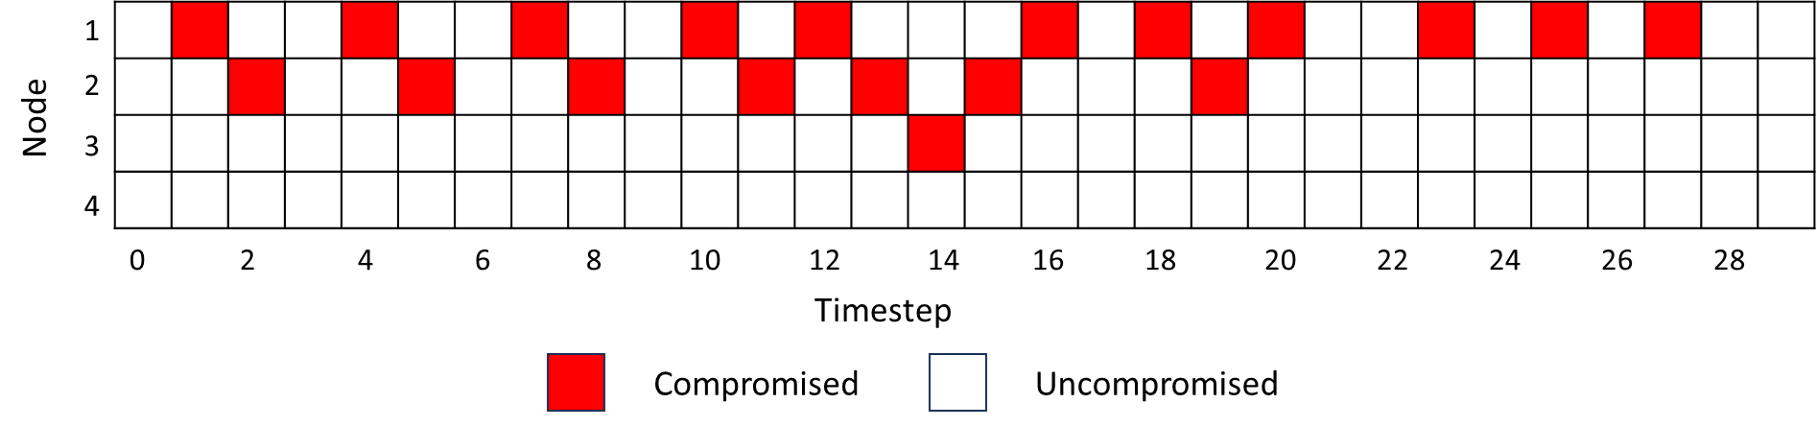
\includegraphics[width=0.9\textwidth]{Images/Comp_status.png}
}

\centering

\subfloat[Node vulnerability]{%
    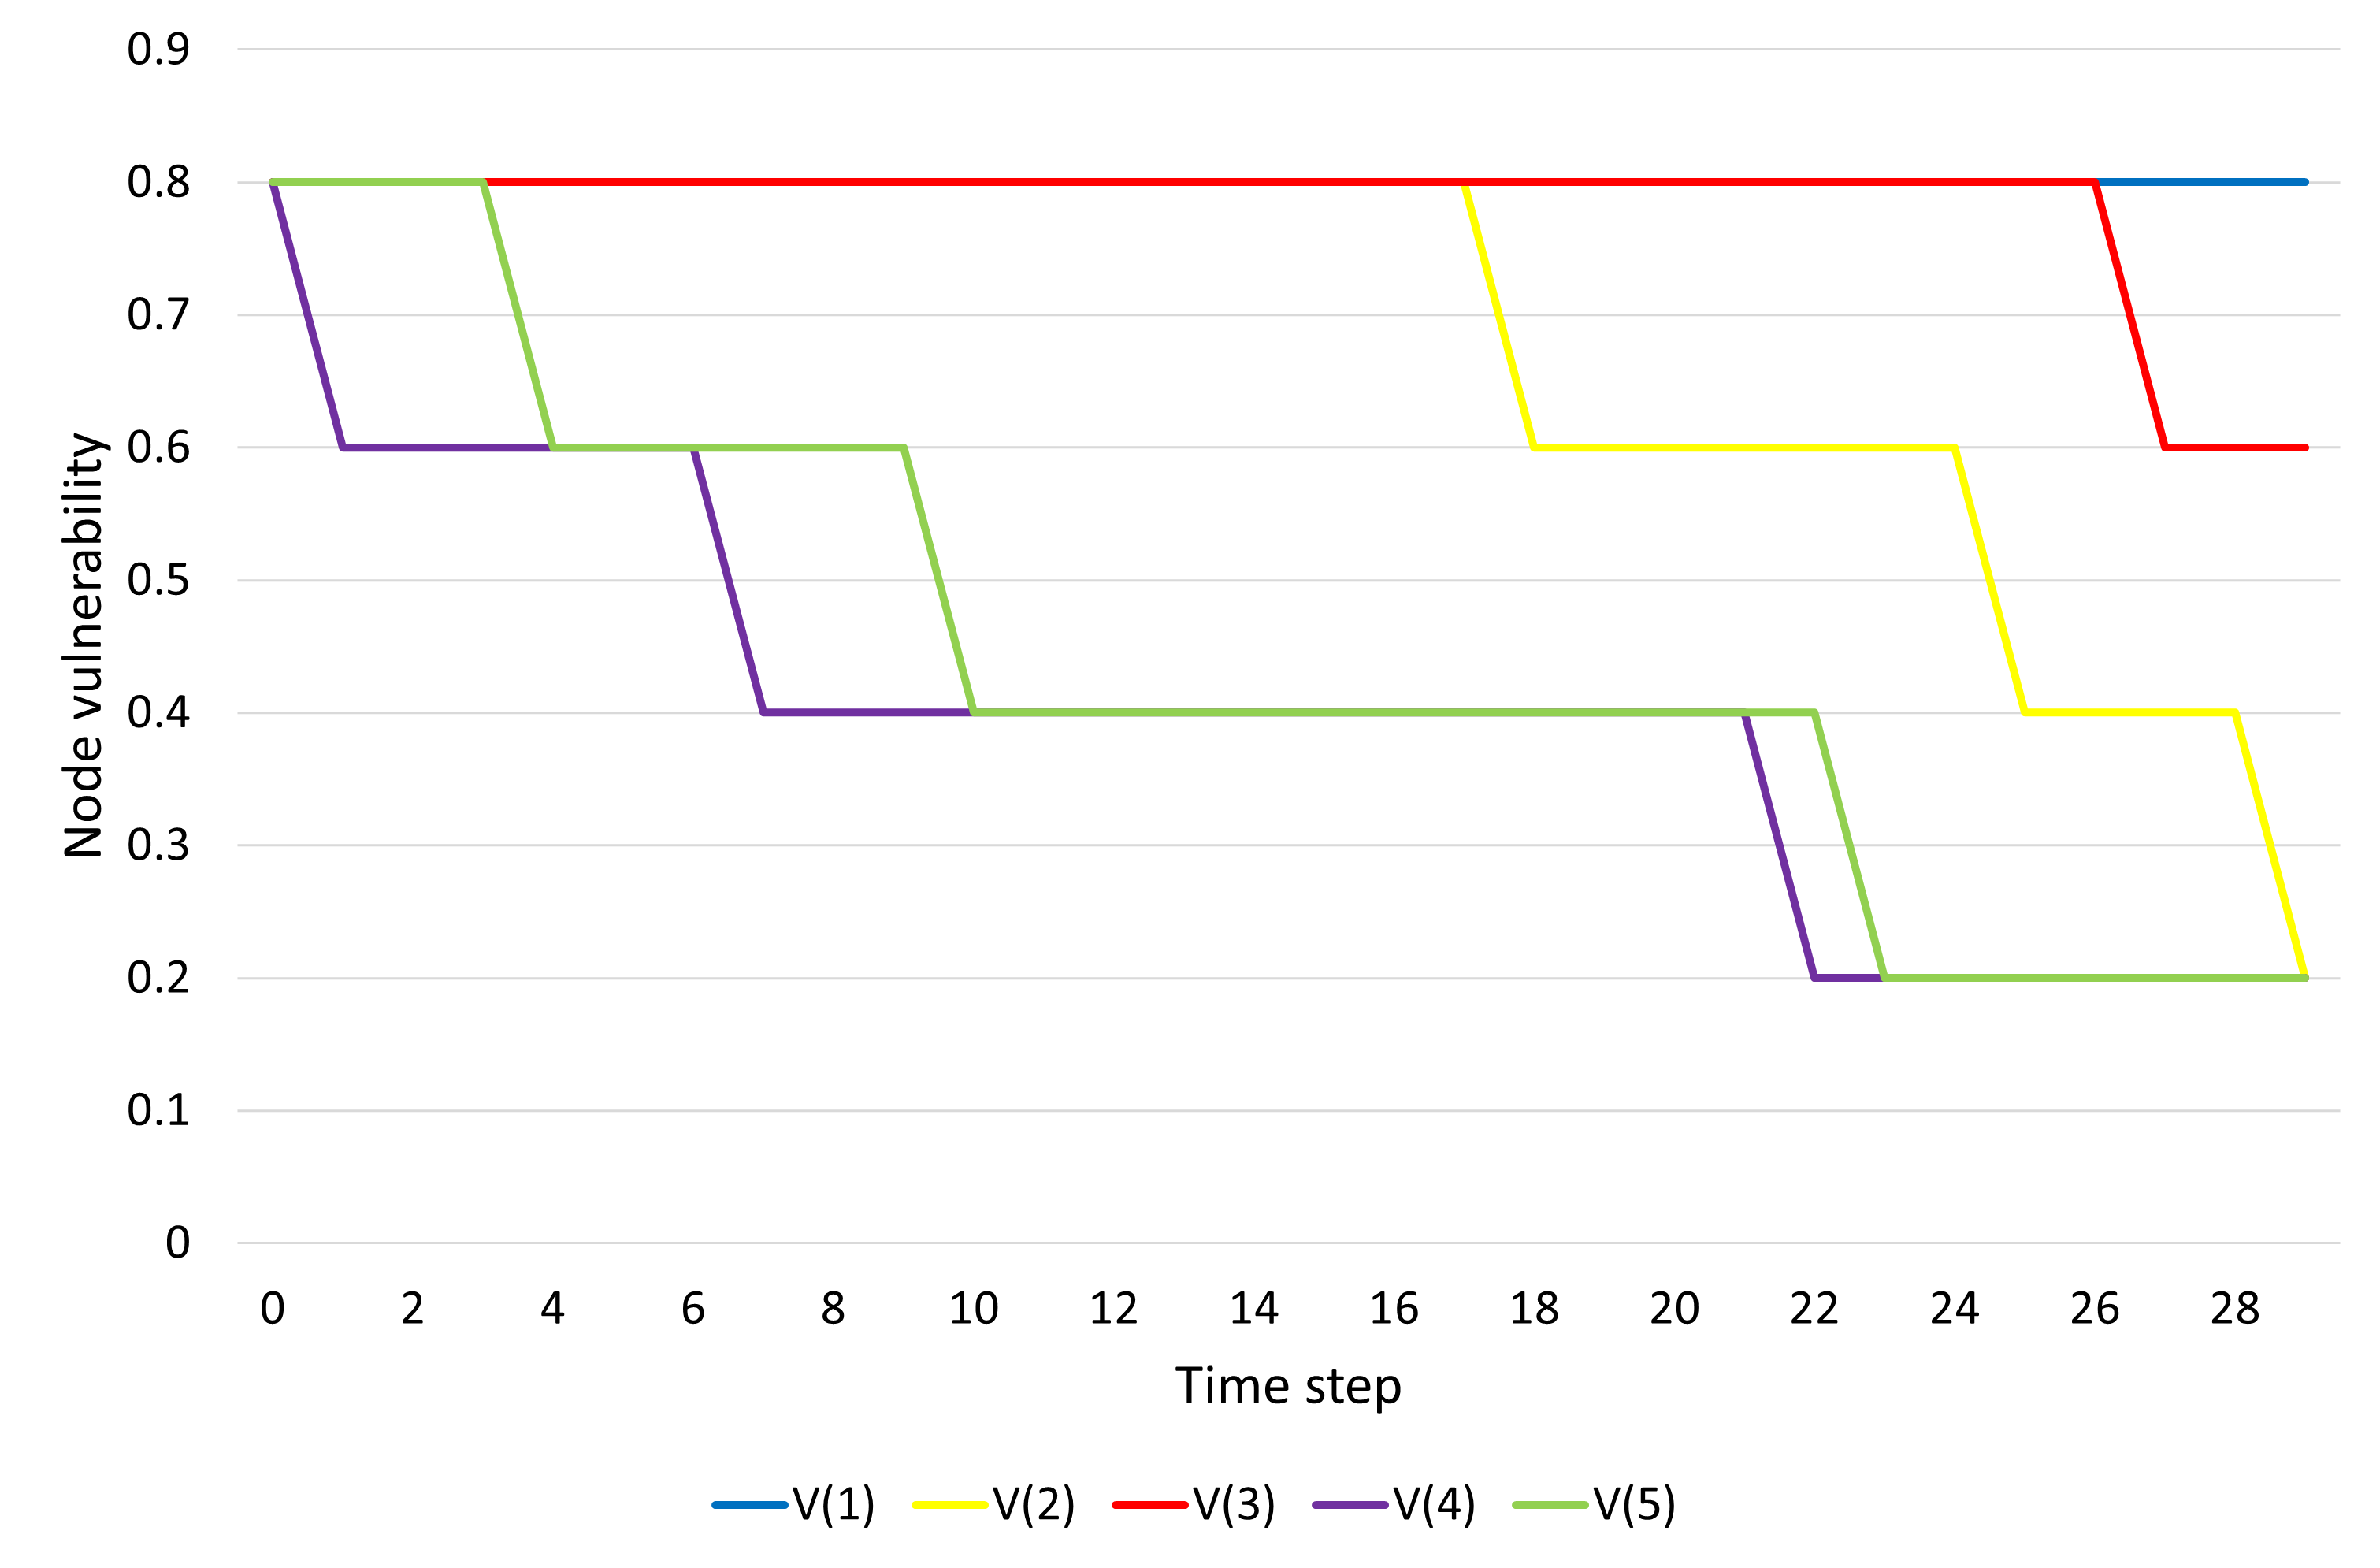
\includegraphics[width=0.9\textwidth]{Images/Node_vulnerabilities.png}
}

\label{fig: YT trajectory}
\caption{A visualisation of the YT trajectory collected for evaluation. Part (a) illustrates the compromise status of each node; time steps at which a node is compromised are represented by a red square in the corresponding box. It is evident that a maximum of one node was compromised at any time step, and node 4 was never compromised. Part (b) displays the node vulnerability values, which all begin at 0.8 as described in the initial YT setup in Section 4. }
\label{fig: YT trajectory}

\end{figure}

\begin{figure}[htp]
    \centering
    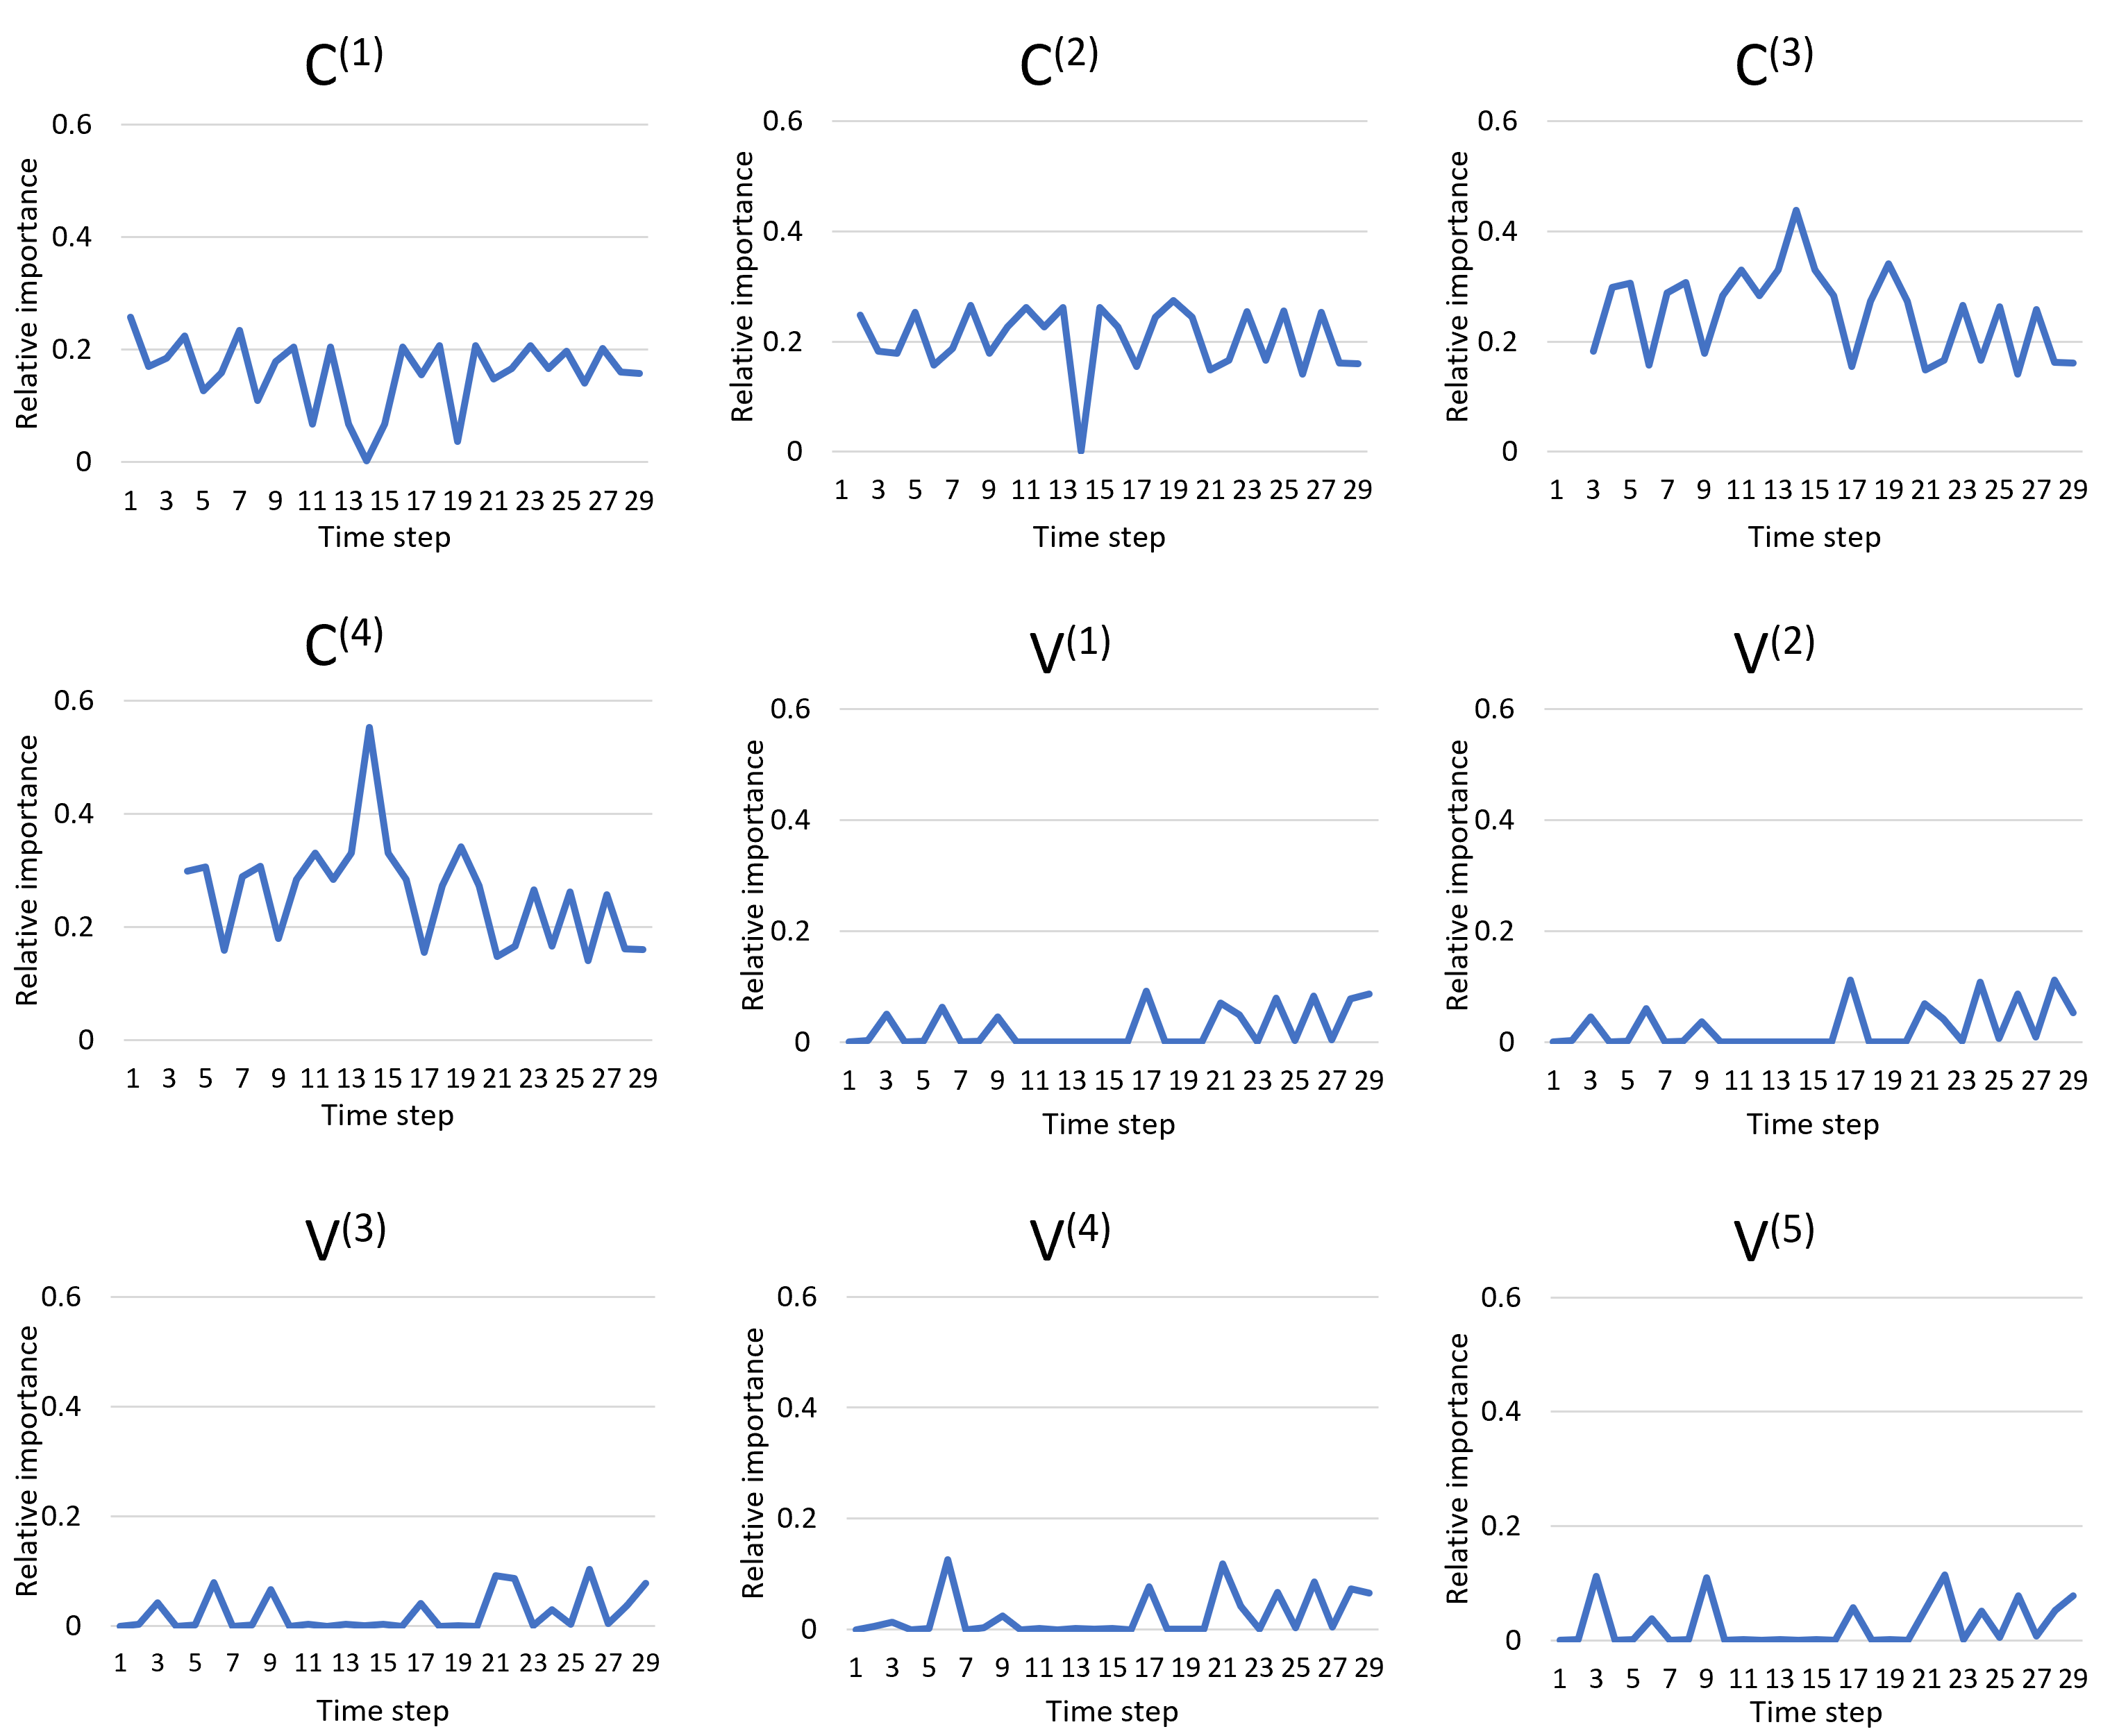
\includegraphics[width=1.0\textwidth]{Images/Importance_graphs.png}
    \caption{A temporal importance plot for each state variable in the considered YT trajectory. Here, the weights calculated using Equation \ref{eq: feature importance} have been rescaled to values in [0,1] so that we can compare the relative importance of each state variable on the action taken by the PPO agent at each time step. Notable events include the compromise of node 3 at time step 14, which corresponds to a peak in the importance plots for $C^{(3)}$ and $C^{(4)}$, while the importance of $C^{(1)}$ and $C^{(2)}$ drops. Further, note that the peaks in the importance graphs for node vulnerabilities correspond perfectly to times at which no node in the network is compromised, as shown in Figure \ref{fig: YT trajectory}.}
    \label{fig: Importance graphs}
\end{figure}

%% bar 17 
\begin{figure}

\centering

\subfloat[YT environment state at step 14 ]{%
    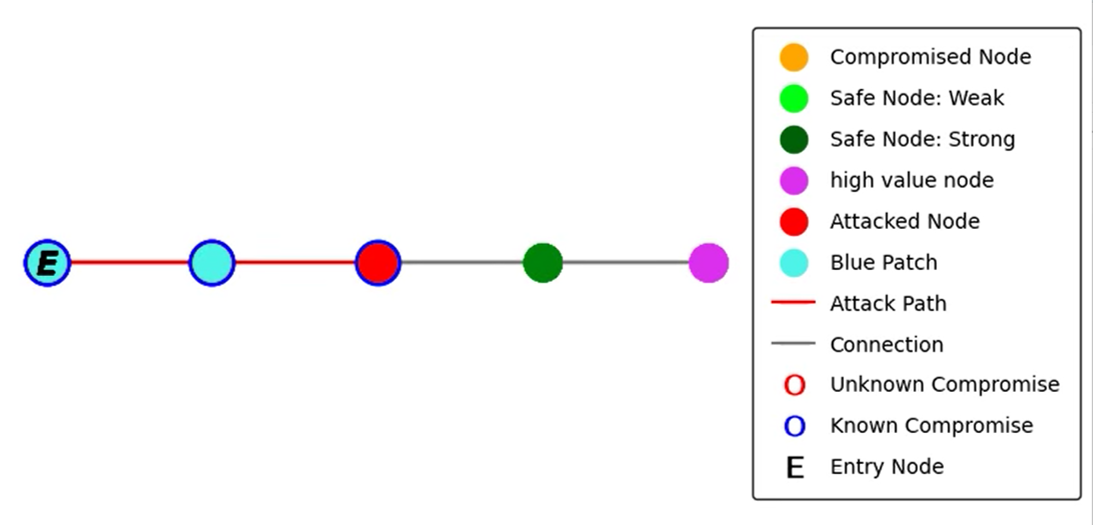
\includegraphics[width=0.9\textwidth]{Images/YT_17.png}
}

\centering

\subfloat[Feature importances for action 14]{%
    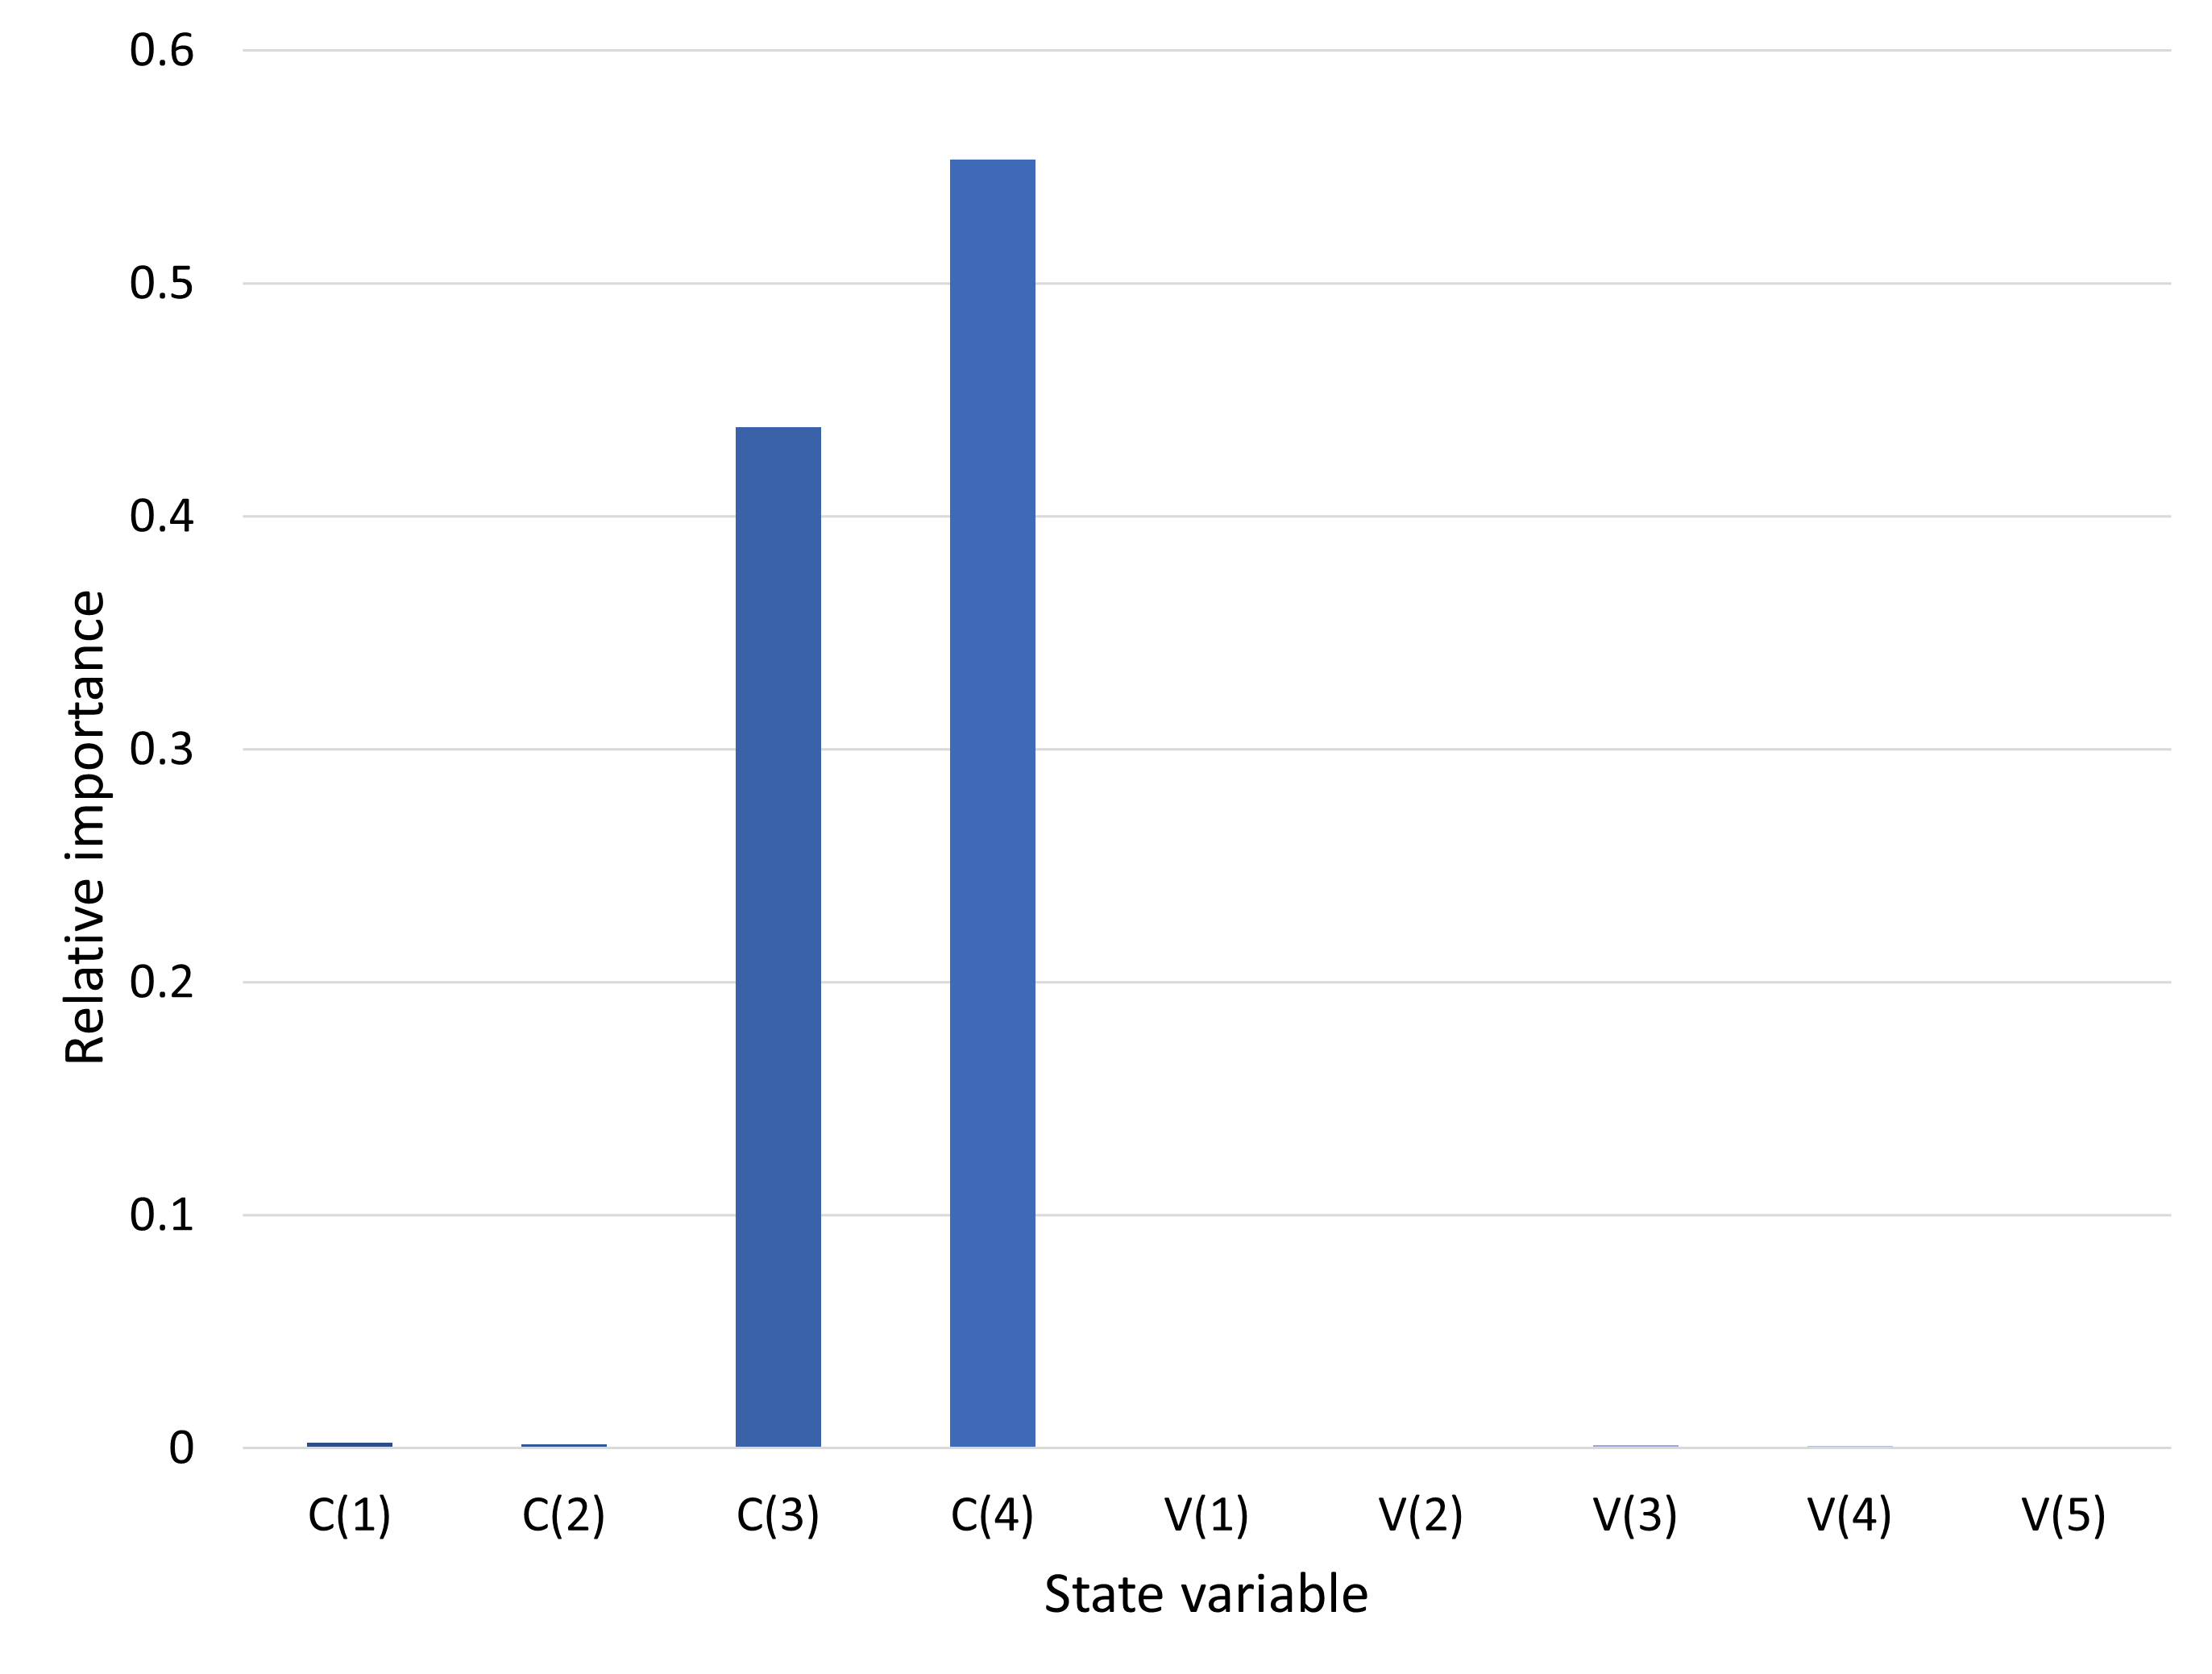
\includegraphics[width=0.9\textwidth]{Images/bar_state_14.png}
}

    \caption{An explanation as to the choice of action `patch node 3' taken by the agent at time step 14. Part (a) gives a visualisation of the state of the YT network at the start of turn 14, and part (b) provides a plot of the corresponding relative feature importances from Figure \ref{fig: Importance graphs}. Together, these show that the action `patch node taken' was taken almost completely due to the fact that node 3 was compromised and node 4 was uncompromised at time 14.}
    \label{fig: state_14}
\end{figure} 



%% bar 21 
\begin{figure}

\centering

\subfloat[YT environment state at step 21 ]{%
    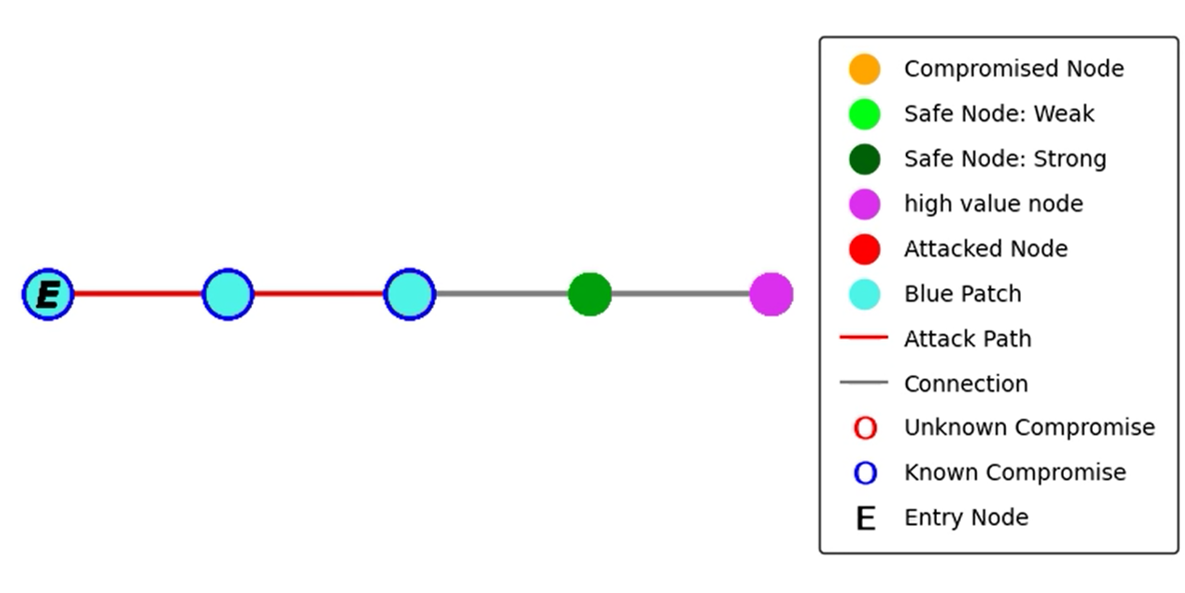
\includegraphics[width=0.9\textwidth]{Images/YT_21.png}
}

\centering

\subfloat[Feature importances for action 21]{%
    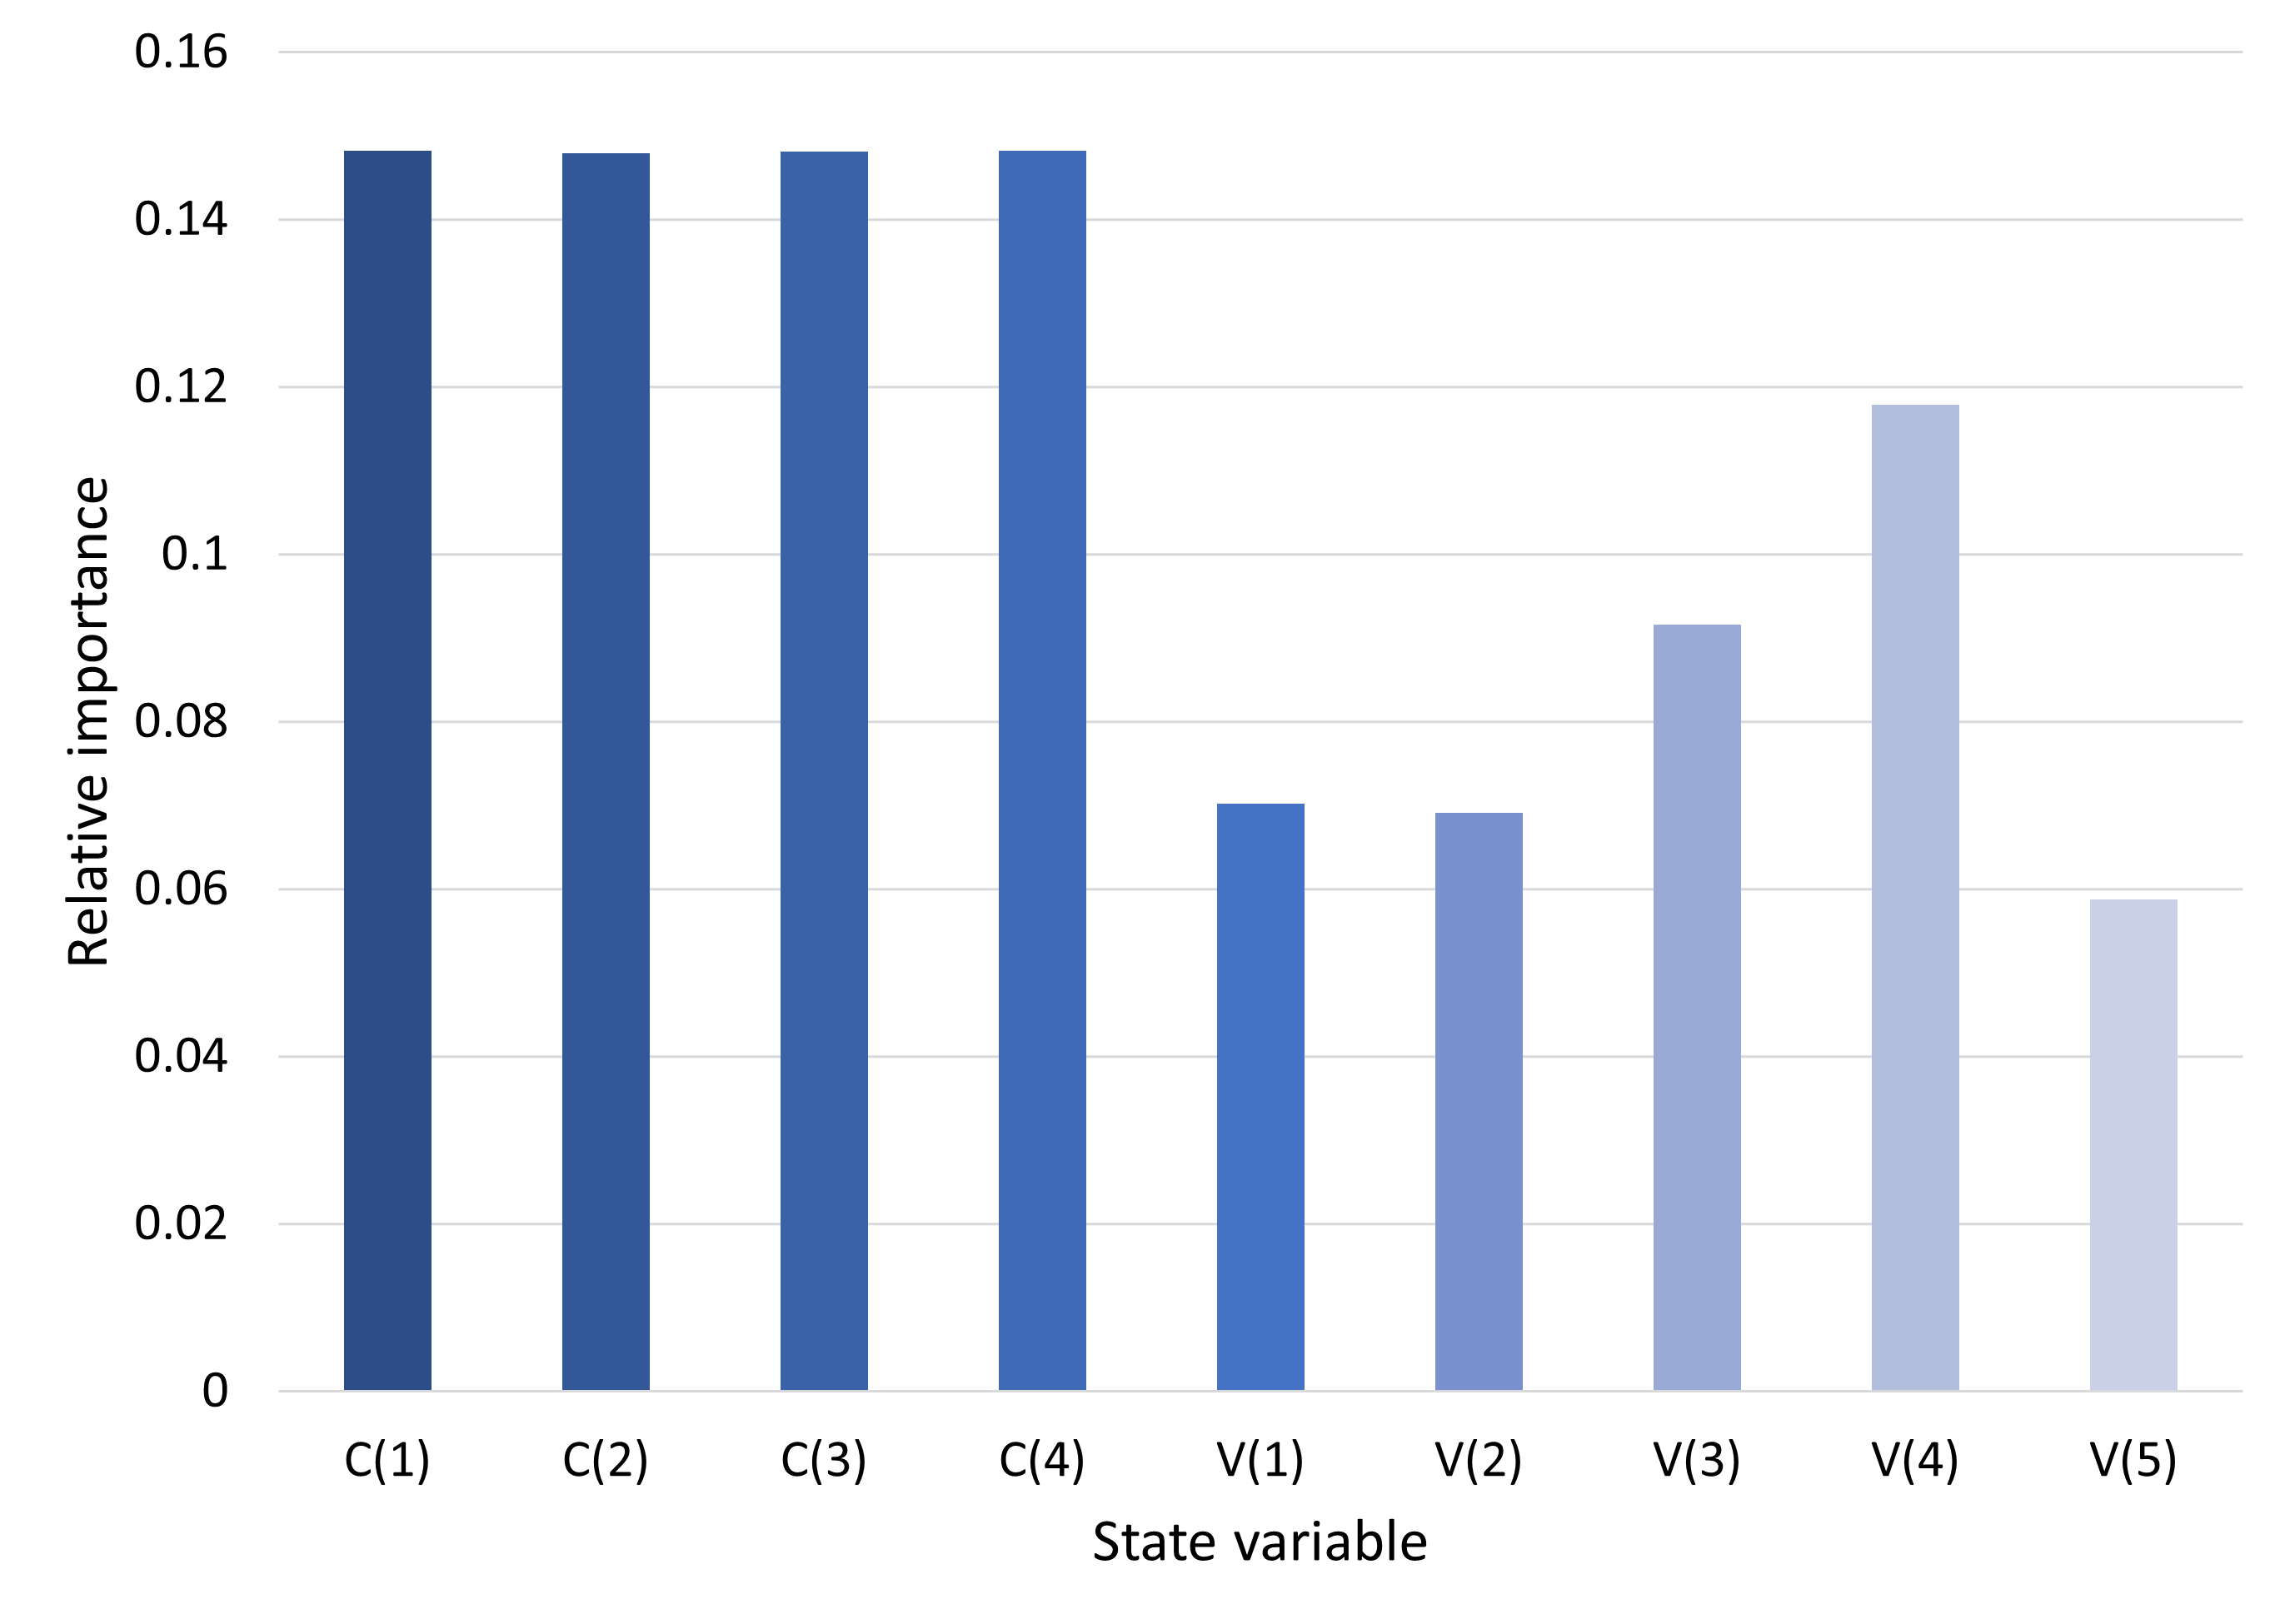
\includegraphics[width=0.9\textwidth]{Images/bar_state_21.png}
}

    \caption{An explanation as to the choice of action `reduce vulnerability of node 4' taken by the agent at time step 21. Part (a) gives a visualisation of the state of the YT network at the start of turn 21, and part (b) provides a plot of the corresponding relative feature importances from Figure \ref{fig: Importance graphs}. Together, these figures show that the fact that all nodes are uncompromised had a large influence on the agent's decision of action. Of the vulnerabilities, we can see that vulnerability of node 4 had the greatest influence over the choice of action, however each is accountable for over 5\% of the choice, implying that the choice of which node's vulnerability to reduce depends on their specific values. In particular, if any vulnerability score had been different then a different action may have been taken at turn 21.}
    \label{fig: state_21}
\end{figure} 


% --------------------------------------------------------

\pagebreak

\section{Conclusions} 

\subsection{Contribution}
This paper has explored the application of causal explanation generation to the problem of understanding the behaviour of autonomous cyber defence agents, trained using Deep Reinforcement Learning. 

First, I conducted a review of the current state of XRL research with particular emphasis on post-hoc explanation generations, and identified limitations of works in the field. I placed particular emphasis on methods incorporating causality so as to emphasise the benefits it can yield with regard to producing human-understandable explanations and models which cannot be misled by spurious correlations. To this end, I presented in detail the three most prominent papers featuring causal explanation mechanisms in order to demonstrate the novelty of such techniques and the challenges associated with such methods. 

In the second part of this paper, I present an adaptation of the causal importance method in \cite{wang2022causal} tailored specifically for a simple YAWNING TITAN cyber simulation scenario. This mechanism learns the structural equations of an SCM and uses them to evaluate counterfactual instances, in order to generate local explanation of agent behaviour. The method is evaluated via a sample trajectory, and examples of the caliber of insight which can be derived from such causal importance values are demonstrated in Section 6. In particular, I produced illustrative plots, which viewed alongside representations of the environment state, provide valuable insights into the influence of each observed variable on the blue agent's choice of action. 


\subsection{Limitations and further work}

In this work, I considered a highly specific and simplified configuration within the YT environment. An immediate extension to this work is to investigate the causal importance method in scenarios with different parameters in order to enhance the applicability of the method to more complex environments. In particular, different network topologies could be explored, and the observation and action spaces broadened, allowing for more defensive actions such as the ability to isolate and reconnect nodes. Other YT capabilities, such as only allowing the blue agent a partial view of the compromised status of nodes and introducing a blue scan action, could also be incorporated to provide a more representative cyber defence scenario. However, the scalability of the approach discussed to more complex scenarios is limited by the need for a pre-determined causal diagram. As discussed in Section 3.4, this is common amongst causal explanation generation techniques, and in the future it would be useful to study how such methods can be used in combination with causal discovery techniques in order to alleviate this assumption. 


Other possibilities for further work include investigating variations to the weighting calculation method, such as altering the vector norm and perturbation values used in Equation (\ref{eq: feature importance}), and comparing the utility of classifiers for approximating the structural equations. It would also be interesting to apply the final part of the method used in \cite{wang2022causal} to the YT scenario, where the causal model is cascaded to gain insight into the influence of past states and actions on the current action.

Finally, this work, as with many of the studies discussed in Section 3, suffers from a lack of user testing. In order to truly evaluate the efficacy of the proposed method for providing human-understandable insight into the reasons behind agent actions, a comprehensive human study needs to be performed, and the method compared with other techniques. As discussed in Section 3.4, more work is needed in the field of XRL in general to build benchmarks for explanation generation by which to evaluate such techniques.


\pagebreak

\section{References}
%\bibliographystyle{unsrt}
%\bibliography{report}


\printbibliography[heading=none, stylename = plain]

\end{document}
